\documentclass[aps,prd,twocolumn,10pt,superscriptaddress,nofootinbib,longbibliography,floatfix]{revtex4-2}

\usepackage{amsmath,amssymb,amsfonts}
\usepackage{bm}
\usepackage{graphicx}
\usepackage{booktabs}
\usepackage{xcolor}
\usepackage{hyperref}
\graphicspath{{figures/}}
\hypersetup{colorlinks=true,linkcolor=blue,citecolor=blue,urlcolor=blue}

\newcommand{\dd}{\mathrm{d}}
\newcommand{\Nppc}{N_{\rm ppc}}
\newcommand{\lcap}{\ell_{\rm cap}}
\newcommand{\aexc}{\alpha_{\rm exc}}
\newcommand{\Ham}{\mathcal{H}}
\newcommand{\Mom}{\mathcal{M}}
\newcommand{\Egeo}{\mathcal{E}}
\newcommand{\Et}{\tilde{E}}
\newcommand{\Bt}{\tilde{B}}
\newcommand{\rbar}{\bar{r}}

\begin{document}

\IfFileExists{sections/title.tex}{% Title block. The abstract below is the writer's 300-word version of the paper and is
% provisional; the final abstract is written last.
\title{Numerical-relativity particle-in-cell method at low particle number:\\ An independent reconstruction by language-model agents}

\author{Author list to be set}
\noaffiliation

\date{Draft of 13 November 2026}

\begin{abstract}
\textit{Provisional abstract of a draft in progress; results marked [pending] were not final when it was written.}
Collisionless matter near black holes obeys the Einstein-Vlasov system, where particles follow geodesics of their curvature. Wu and Most introduced a numerical-relativity particle-in-cell method with millions of phase-space packets called macroparticles. We ask whether their text enables an independent rebuild and what changes at ten thousand macroparticles. Language-model agents under human direction built the code from text alone in AthenaK, with separate models for code, checks, and writing. Predictions written before each control run tested every diagnosis. Each step evolves spacetime like a field solver, advances macroparticles by a pusher, and spreads sources onto cells by cloud-in-cell deposition. The implicit midpoint pusher matches Kerr orbits, while the spacetime Boris pusher needs an unstated local-frame tetrad gauge: symmetric analytically, Cholesky on meshes. Tracers near fixed and evolving black holes conserve invariants, and deposition conserves sources across refinement. Geometric slice-mass checks of apparent horizons, outermost surfaces of non-expanding light rays, exposed an unfilled ghost-cell defect in AthenaK's apparent-horizon finder. Interpolant derivatives agree within the accuracy of the mass measure. Surface mass rescaling removes dust-collapse lattice excess at ten thousand macroparticles. A filter compensation pass cancels cloud widening that expands stable clusters. Level-capped deposition coarsens clouds yet worsens constraints and apparent-horizon mass drift near black holes, so finest-level deposition stays. Dust collapses to a black hole of matching apparent-horizon mass while lapse excision removes interior particles frozen by time dilation. Monoenergetic clusters, equal-energy stellar spheres, stay bound with a growing core oscillation. The cause of that growth and coarsened-cloud drift is not determined. Past the binding-energy maximum, unperturbed unstable clusters expand toward migration [pending], perturbed ones collapse [pending], and unbound ones disperse [pending]. Prolate clouds collapse [pending], and a relativistic cluster with two collapsing overdensities at speed-consistent radius merges [pending]. These controls establish a reproducible algorithm: ten thousand macroparticles capture black hole formation and cluster stability.
\end{abstract}

\maketitle
}{}

\IfFileExists{sections/introduction.tex}{\section{Introduction}\label{sec:intro}

Stars in dense relativistic clusters and collisionless dark matter around black holes move freely through collective gravitational fields that vary strongly in space and time \cite{1985ApJ...298...34S,2008gady.book.....B,Andreasson:2011ng,Angulo:2021kes,Bamber:2025gxj}. Two-body gravitational encounters act over timescales far longer than a dynamical crossing time, much as binary collisions remain negligible in a collisionless plasma \cite{1991ppcs.book.....B,2008gady.book.....B}. Multi-stream trajectories cross in configuration space and build anisotropic stresses, whereas single-fluid hydrodynamics assigns one bulk velocity to each spatial point \cite{Andreasson:2011ng,East:2019chx}. Strong-field evolution therefore requires the Einstein-Vlasov system, a phase-space kinetic description coupled to the full Einstein equations where matter follows geodesics of the curvature its stress-energy generates \cite{Andreasson:2011ng,Sarbach:2013fya,Acuna-Cardenas:2021nkj}. Early numerical studies with spherical codes mapped equilibrium sequences, radial stability, and black hole formation in relativistic clusters \cite{1968ApJ...154..251I,1980ApJ...238.1101I,1985ApJ...298...34S,1985ApJ...298...58S} alongside critical gravitational collapse \cite{Rein:1998uf,Olabarrieta:2001wy,Akbarian:2014gna}. Subsequent axisymmetric and three-dimensional simulations extended kinetic gravity to rotating clusters, nonspherical collapse, and cosmic structure \cite{Abrahams:1994ge,Shibata:1999va,Shibata:1999wi,East:2019bwu,East:2019chx,Ames:2020ssl}, where asymmetric instabilities and mergers demand evolution in three spatial dimensions.

The numerical-relativity particle-in-cell (NRPIC) method of Ref.~\cite{Wu:2026nrpic} brings algorithms from relativistic plasma simulation \cite{1988csup.book.....H,1991ppcs.book.....B,Spitkovsky:2005vsy,Cerutti:2013mma,EntityDevelopmentTeam:2025tlp} to three-dimensional Einstein-Vlasov evolution. Macroparticles---finite-mass packets sampling six-dimensional phase space---advance along timelike geodesics through a time-reversible trajectory pusher in the reconstructed metric \cite{boris1970relativistic,Bacchini:2020cze,Olivares:2021cfa,Boyeneni:2025tsx,Wu:2026nrpic}. Conservative cloud-in-cell deposition assigns each macroparticle's energy, momentum, and stress to nearby mesh cells across refinement boundaries before grid filtering smooths discrete sampling noise \cite{1988csup.book.....H,1991ppcs.book.....B,Myers:2021gfn,Wu:2026nrpic}. A constraint-damped solver in moving-puncture gauge, the standard way to evolve Einstein's equations through black hole formation on a fixed grid, advances the spacetime on an adaptive mesh \cite{Bona:2003fj,Campanelli:2005dd,Baker:2005vv,Hilditch:2012fp,Wu:2026nrpic}. Reference~\cite{Wu:2026nrpic} demonstrated this coupled cycle on gravitational collapse and relativistic cluster benchmarks using millions of macroparticles on large machines.

Two questions decide how broadly this method can be adopted. One question asks whether an independent builder without access to the original code can reconstruct the NRPIC method quantitatively from its published description alone. A numerical method is usable by others only when its written equations and algorithmic rules suffice for an independent implementation to recover its benchmarks. The second question asks which results survive at ten thousand macroparticles, where a run takes minutes to a few hours on one graphics card, and what must change for that. A small computational entry cost decides who can use the method for routine physical exploration, rapid parameter surveys, and independent verification.

Language-model agents under human direction built an independent implementation from the published text alone inside the public AthenaK code \cite{2026ApJS..283...27S,Zhu:2024utz}, with portable parallel execution through Kokkos \cite{2022ITPDS..33..805T}. Every algorithmic stage and coupled test was compared with exact analytical solutions or with the published numbers of Ref.~\cite{Wu:2026nrpic}. Candidate explanations of unexpected results were tested against predictions recorded before control runs designed so that they could fail, as described in Sec.~\ref{sec:assembly}.

The published description suffices to rebuild the method and reproduce the single-particle errors of Ref.~\cite{Wu:2026nrpic} once one unstated choice is identified (Sec.~\ref{sec:testparticles}). That choice is the tetrad gauge, the local rotation freedom of the orthonormal frame in the spacetime Boris pusher, where distinct frame constructions shift the discrete error (Secs.~\ref{sec:pushers} and \ref{sec:testparticles}). Self-gravitating evolutions at ten thousand macroparticles require two algorithmic changes (Sec.~\ref{sec:selfgravity}). Surface masses on a cubic dust lattice must be rescaled because discrete site counts inside a sphere exceed its continuum volume at low particle number (Sec.~\ref{sec:dust}). Multi-pass source filters require a sharpening compensation pass \cite{1991ppcs.book.....B} because plain smoothing widens clouds like gravitational softening and makes stable clusters bounce outward (Secs.~\ref{sec:deposition} and \ref{sec:clusters}). Coarser particle clouds---a tempting change on sparse refined meshes---raise constraint violations and drive black hole mass drift, so clouds belong on the finest local level (Sec.~\ref{sec:selfgravity}). A geometric mass measure of the slice also exposed a ghost-zone defect in the host code's finder for apparent horizons, the outermost closed surfaces of zero outgoing light expansion (Secs.~\ref{sec:numerical_methods} and \ref{sec:dust}). With these elements in place, ten thousand macroparticles reproduce in kind dust collapse \cite{Oppenheimer:1939ue}, the sequence of relativistic clusters \cite{1985ApJ...298...34S,1985ApJ...298...58S}, and the migration of an unstable cluster toward the stable branch \cite{Font:2001ew,Wu:2026nrpic} (Secs.~\ref{sec:dust} and \ref{sec:clusters}). Documented differences from Ref.~\cite{Wu:2026nrpic} appear in the collapse times of unstable clusters and in the collapse of one perturbed near-critical model (Sec.~\ref{sec:clusters}).

Section~\ref{sec:system} formulates collisionless matter in a dynamical spacetime and its macroparticle phase-space representation. Section~\ref{sec:method} presents the particle-mesh method: geodesic pushers, metric reconstruction, stress-energy deposition and filtering, spacetime evolution, adaptive mesh refinement, and numerical methods. Section~\ref{sec:testparticles} tests the geodesic pushers, phase mixing, source conservation, and interior particle removal by lapse excision around fixed and evolving black holes. Section~\ref{sec:selfgravity} studies self-gravitating matter at ten thousand macroparticles across spherical dust collapse and the sequence of relativistic clusters. Section~\ref{sec:assembly} describes how the code was assembled and verified, before the final section states our conclusions and the appendix records the scenario parameters.
}{}
\IfFileExists{sections/system.tex}{\section{Collisionless matter in a dynamical spacetime}\label{sec:system}

Stars in dense clusters, particles in dark-matter spikes, and debris in colliding stellar streams move freely through smooth collective gravitational fields \cite{1985ApJ...298...34S,2008gady.book.....B,Andreasson:2011ng}. Two-body gravitational encounters act over timescales far longer than a dynamical crossing time, so each constituent follows a geodesic of the spacetime geometry generated by the whole ensemble. Throughout this paper we set Newton's gravitational constant $G$ and the speed of light $c$ to unity and adopt metric signature $(-,+,+,+)$. Greek letters $\mu,\nu,\rho,\sigma$ label spacetime indices, Latin letters $i,j,k,l$ label spatial coordinate indices, and parenthesized indices $(m),(n),(k)$ label components in a tetrad, a local frame of four mutually perpendicular unit vectors.

Collisionless matter in a curved spacetime with metric $g_{\mu\nu}$ and inverse $g^{\mu\nu}$ is described in phase space by a rest-mass-weighted distribution function $f(x^\mu, u^\nu)$ \cite{Andreasson:2011ng,Sarbach:2013fya,Acuna-Cardenas:2021nkj}. Here $x^\mu$ are spacetime coordinates and $u^\mu$ is the four-velocity, equal to the four-momentum per unit rest mass on the future mass shell $g_{\mu\nu} u^\mu u^\nu = -1$. Phase-space conservation along free-fall worldlines coupled to Einstein's field equations forms the Einstein-Vlasov system,
\begin{align}\label{eq:einstein_vlasov}
u^\mu \partial_\mu f - \Gamma^\mu_{\nu\rho} u^\nu u^\rho \frac{\partial f}{\partial u^\mu} &= 0, \nonumber\\
G_{\mu\nu} &= 8\pi T_{\mu\nu},
\end{align}
where $\Gamma^\mu_{\nu\rho}$ are the Christoffel symbols of $g_{\mu\nu}$. The Einstein tensor $G_{\mu\nu}$ is sourced by the stress-energy tensor $T_{\mu\nu}$, given by the second four-velocity moment of $f$ over the future mass shell.

Time evolution splits the spacetime into spacelike hypersurfaces of constant coordinate time $t$ with spatial coordinates $x^i$, induced metric $\gamma_{ij}$, inverse $\gamma^{ij}$, and determinant $\gamma = \det(\gamma_{ij})$ \cite{Arnowitt:1962hi}. Local measurements on each slice are referred to normal observers, Eulerian observers whose worldlines cross the slice orthogonally with future-directed unit four-velocity $n^\mu$ and covector $n_\mu = (-\alpha, 0, 0, 0)$. The lapse $\alpha$ links adjacent slices by converting a coordinate interval $\dd t$ into proper time $\alpha\,\dd t$ along normal observers. The shift $\beta^i$ gives the coordinate velocity at which spatial grid points drift relative to those normal observers. In these variables the spacetime line element reads
\begin{equation}\label{eq:line_element}
\dd s^2 = -\alpha^2\,\dd t^2 + \gamma_{ij}(\dd x^i + \beta^i\,\dd t)(\dd x^j + \beta^j\,\dd t),
\end{equation}
with $n^\mu = (\alpha^{-1}, -\alpha^{-1}\beta^i)$. The bending of each slice inside the ambient spacetime is measured by the symmetric extrinsic curvature $K_{ij}$, defined through
\begin{equation}\label{eq:extrinsic_curvature}
\partial_t \gamma_{ij} = -2\alpha K_{ij} + D_i \beta_j + D_j \beta_i,
\end{equation}
where $D_i$ is the spatial covariant derivative compatible with $\gamma_{ij}$ and $\beta_i = \gamma_{ij}\beta^j$. Normal observers project $T^{\mu\nu}$ into ten matter fields---the energy density $E$, covariant momentum density $S_i$, and symmetric spatial stress $S_{ij}$---according to
\begin{align}\label{eq:source_projections}
E &= n_\mu n_\nu T^{\mu\nu}, &
S_i &= -g_{i\mu} n_\nu T^{\mu\nu}, \nonumber\\
S_{ij} &= g_{i\mu} g_{j\nu} T^{\mu\nu}. & &
\end{align}

Direct grid discretization of $f$ spans six phase-space dimensions and becomes prohibitive in three spatial dimensions without symmetry, whereas the Vlasov equation conserves phase-space weight along timelike geodesics. A particle-in-cell method \cite{1988csup.book.....H,1991ppcs.book.....B,Wu:2026nrpic} exploits these characteristics by sampling $f$ with $N$ finite-weight phase-space packets called macroparticles, indexed by $p = 1, \dots, N$. With $u_\mu = g_{\mu\nu} u^\nu$, each macroparticle carries fixed rest mass $m_p$, spatial coordinates $x_p^i(t)$, and covariant spatial four-velocity components $u_{i,p}(t) = g_{i\mu} u_p^\mu$, giving six phase-space variables per particle. On the future mass shell $g^{\mu\nu} u_\mu u_\nu = -1$, the Lorentz factor seen by normal observers is
\begin{equation}\label{eq:lorentz_factor}
W = \alpha u^0 = \sqrt{1 + \gamma^{ij} u_i u_j},
\end{equation}
which determines the single-particle Hamiltonian $-u_0 = \alpha W - \beta^i u_i$. Hamilton's canonical equations for $(x^i, u_i)$ yield the characteristic equations,
\begin{align}\label{eq:characteristics}
\frac{\dd x^i}{\dd t} &= \frac{\alpha \gamma^{ij} u_j}{W} - \beta^i, \nonumber\\
\frac{\dd u_i}{\dd t} &= -W \partial_i \alpha + u_j \partial_i \beta^j - \frac{\alpha}{2W} u_j u_k \partial_i \gamma^{jk}.
\end{align}
At spatial coordinate $\bm{x} = (x^1, x^2, x^3)$, the ensemble stress-energy projected onto normal observers forms the particle sources,
\begin{align}\label{eq:particle_sources}
E(t,\bm{x}) &= \sum_{p=1}^{N} \frac{m_p W_p}{\sqrt{\gamma}}\,\delta^3(\bm{x} - \bm{x}_p), \nonumber\\
S_i(t,\bm{x}) &= \sum_{p=1}^{N} \frac{m_p u_{i,p}}{\sqrt{\gamma}}\,\delta^3(\bm{x} - \bm{x}_p), \nonumber\\
S_{ij}(t,\bm{x}) &= \sum_{p=1}^{N} \frac{m_p u_{i,p} u_{j,p}}{W_p \sqrt{\gamma}}\,\delta^3(\bm{x} - \bm{x}_p).
\end{align}
Here $\delta^3(\bm{x} - \bm{x}_p)$ is the three-dimensional coordinate Dirac distribution and $W_p$ is evaluated at $\bm{x}_p(t)$. Geodesic transport of $(x_p^i, u_{i,p})$ under the characteristic equations, coupled to smoothed mesh projections of the particle sources, solves the Einstein-Vlasov system.
}{}
\IfFileExists{sections/method.tex}{\section{The particle-mesh method}\label{sec:method}

Evolving collisionless matter in dynamical gravity requires advancing smooth curvature fields on an Eulerian mesh alongside discrete phase-space trajectories over a shared global time step $\Delta t$, set by the Courant limit of the finest cell spacing $\Delta x$, without updating the particle ensemble at every intermediate substep of the field equations. The numerical-relativity particle-in-cell (NRPIC) method \cite{Wu:2026nrpic} couples the two representations through a staggered cycle in which a hyperbolic spacetime solver---the gravitational counterpart of the Maxwell solver in an electromagnetic particle-in-cell code \cite{1988csup.book.....H,1991ppcs.book.....B}---evolves cell-centered metric fields while macroparticles follow geodesics and return smoothed stress-energy moments to the grid. Representing phase space with a mean count $\Nppc$ of macroparticles per cell introduces discrete sampling noise of relative amplitude $\Nppc^{-1/2}$, so each stage is built to preserve time-reversal symmetry on orbits, exact integral weight across mesh interfaces, and smooth sources when $\Nppc$ is modest.

One cycle from $t^n$ to $t^{n+1} = t^n + \Delta t$ executes six stages in sequence (Fig.~\ref{fig:cycle}). First, $\alpha$, $\beta^i$, and $\gamma_{ij}$ at $t^n$ are saved across all active and ghost cells so trajectories can access both endpoints of the step. Second, holding the sources $(E, S_i, S_{ij})$ deposited at $t^n$ fixed across four fourth-order Runge--Kutta stages advances the spacetime variables to $t^{n+1}$, supplying the future metric at the cost of a single particle update per step. Third, a geodesic pusher---an update advancing each macroparticle's position and momentum across $\Delta t$---evolves every particle from $t^n$ to $t^{n+1}$ in the midpoint-averaged metric interpolated between $t^n$ and $t^{n+1}$. Fourth, lapse excision removes particles deep inside black holes where the interpolated initial lapse satisfies $\alpha(t^n, \bm{x}_p^n) < \aexc$ for a threshold $\aexc$, out-of-bounds and nonfinite particles are discarded, and remaining particles are reassigned to their enclosing mesh blocks. Fifth, stress-energy deposition---assigning each macroparticle's mass-energy, momentum, and stress to neighboring cells---builds $(E, S_i, S_{ij})$ at $t^{n+1}$, applies binomial smoothing passes, and evaluates the gravitational constraints with the updated sources. Sixth, diagnostics run and the adaptive mesh refines or coarsens where curvature gradients demand; after any regrid, metric arrays, block ownership, and deposited sources are rebuilt on the new leaf hierarchy while every macroparticle keeps its rest mass $m_p$, position $x_p^i$, and momentum $u_{i,p}$ unchanged.

\subsection{Geodesic pushers}\label{sec:pushers}

Sustaining collisionless equilibria over many crossing times and resolving periapsis passages near spinning black holes require trajectory updates free of secular drift in orbital invariants. Both pushers implemented here---the implicit midpoint pusher and the spacetime Boris pusher \cite{Wu:2026nrpic}---store $x_p^i$ and $u_{i,p}$ at integer time levels, achieve second-order accuracy in $\Delta t$, and maintain time-reversal symmetry through implicit midpoint evaluation. Each queries the geometry solely through a point-evaluation interface returning $\alpha$, $\beta^i$, $\gamma_{ij}$, and their first spatial derivatives, so identical trajectory code runs on analytic metrics in arbitrary coordinates, uniform-lattice samples, and adaptive mesh blocks. Fixed-point iteration updates the six endpoint variables $(x_p^{i,n+1}, u_{i,p}^{n+1})$ until the largest component change falls below a tolerance.

Suppressing the particle index $p$, the implicit midpoint pusher forms the phase-space midpoint
\begin{equation}\label{eq:midpoint_state}
\bar{x}^i = \frac{x^{i,n} + x^{i,n+1}}{2}, \qquad
\bar{u}_i = \frac{u_i^n + u_i^{n+1}}{2},
\end{equation}
and averages the $t^n$ and $t^{n+1}$ spatial reconstructions at $\bar{\bm{x}}$ to obtain $\bar{\alpha}$, $\bar{\beta}^i$, $\bar{\gamma}_{ij}$, and their spatial derivatives. Inverting $\bar{\gamma}_{ij}$ gives $\bar{\gamma}^{ij}$, $\bar{u}^i = \bar{\gamma}^{ij}\bar{u}_j$, and $\bar{W} = \sqrt{1 + \bar{\gamma}^{ij}\bar{u}_i\bar{u}_j}$, advancing the trajectory by the midpoint update,
\begin{align}\label{eq:midpoint_update}
\frac{x^{i,n+1} - x^{i,n}}{\Delta t} &= \frac{\bar{\alpha}\bar{\gamma}^{ij}\bar{u}_j}{\bar{W}} - \bar{\beta}^i, \nonumber\\
\frac{u_i^{n+1} - u_i^n}{\Delta t} &= -\bar{W}\partial_i\bar{\alpha} + \bar{u}_j\partial_i\bar{\beta}^j + \frac{\bar{\alpha}}{2\bar{W}}\bar{u}^j\bar{u}^k\partial_i\bar{\gamma}_{jk},
\end{align}
where $\bar{u}^j\bar{u}^k\partial_i\bar{\gamma}_{jk} = -\bar{u}_j\bar{u}_k\partial_i\bar{\gamma}^{jk}$. Fixed uniquely by the coordinate metric, the midpoint update conserves any momentum $u_i$ conjugate to a cyclic coordinate ($\partial_i = 0$) to rounding error \cite{Bacchini:2020cze}.

The spacetime Boris pusher projects the momentum onto a tetrad, a local orthonormal frame of four mutually perpendicular unit vectors---here $e_{(0)}^\mu = n^\mu$ along the normal observers together with a spatial triad $e^{(m)}_i$ of three mutually perpendicular unit covectors on the slice---in which the metric is locally Minkowskian \cite{Olivares:2021cfa,Boyeneni:2025tsx,Wu:2026nrpic}. The triad and its inverse $e^i_{(m)}$ satisfy
\begin{equation}\label{eq:triad_def}
\gamma_{ij} = \delta_{mn} e^{(m)}_i e^{(n)}_j, \qquad
e^i_{(m)} e^{(n)}_i = \delta^n_m,
\end{equation}
with Kronecker deltas $\delta_{mn}$ and $\delta^n_m$, defining the tetrad momentum $u_{(m)} = e^i_{(m)} u_i$ (so $u_i = e^{(n)}_i u_{(n)}$) and $W = \sqrt{1 + \delta^{mn} u_{(m)} u_{(n)}}$. Along a trajectory with $u^j = \gamma^{jk} u_k$, coordinate velocity $v^j$, and convective derivative
\begin{equation}\label{eq:coord_vel}
\frac{\dd}{\dd t} = \partial_t + v^j \partial_j, \qquad
v^j = \frac{\alpha u^j}{W} - \beta^j,
\end{equation}
differentiating $u_i = e^{(n)}_i u_{(n)}$ yields
\begin{equation}\label{eq:triad_chain}
e^{(n)}_i \frac{\dd u_{(n)}}{\dd t} = \frac{\dd u_i}{\dd t} - u_{(n)}\bigl(\partial_t e^{(n)}_i + v^j \partial_j e^{(n)}_i\bigr).
\end{equation}
Differentiating $\gamma_{jk} = \delta_{mn} e^{(m)}_j e^{(n)}_k$ rewrites the metric-gradient force in the characteristic equations as
\begin{equation}\label{eq:metric_triad_id}
\frac{1}{2} u^j u^k \partial_i \gamma_{jk} = u^j u_{(n)} \partial_i e^{(n)}_j.
\end{equation}
Defining the momentum-contracted triad gradients
\begin{equation}\label{eq:triad_gradients}
c_{jk} = u_{(n)} \partial_j e^{(n)}_k, \qquad
c^t_k = u_{(n)} \partial_t e^{(n)}_k,
\end{equation}
inserting the characteristic equations, contracting with $e^i_{(m)}$, and passing to normal-observer proper time $\dd\hat{t} = \alpha\,\dd t$ gives the tetrad equation of motion,
\begin{equation}\label{eq:tetrad_eom}
\frac{\dd u_{(m)}}{\dd\hat{t}} = \Et_{(m)} + \frac{1}{W}\epsilon_{(m)(n)(k)} u_{(n)} \Bt_{(k)},
\end{equation}
where $\epsilon_{(m)(n)(k)}$ is the Levi-Civita symbol and the momentum-contracted gravito-electric and gravito-magnetic fields $\Et_{(m)}$ and $\Bt_{(k)}$ are
\begin{align}\label{eq:gravito_em}
\alpha \Et_{(m)} &= e^i_{(m)}\bigl(-W\partial_i\alpha + u_j\partial_i\beta^j + \beta^j c_{ji} - c^t_i\bigr), \nonumber\\
\Bt_{(k)} &= \epsilon_{(k)(m)(n)} e^i_{(m)} e^j_{(n)} c_{ij},
\end{align}
representing the tetrad field strengths $\partial_\mu e^{(m)}_\nu - \partial_\nu e^{(m)}_\mu$ contracted with momentum \cite{Olivares:2021cfa,Boyeneni:2025tsx}.

In plasma simulation \cite{boris1970relativistic,1991ppcs.book.....B}, the Boris step splits the Lorentz force into two half-step electric kicks that change particle energy and momentum magnitude, separated by a magnetic rotation at constant Lorentz factor. Here $\Et_{(m)}$---carrying lapse, shift, and temporal triad gradients---drives the energy-changing kicks, while $\Bt_{(k)}$---carrying the spatial curl of the triad---rotates $u_{(m)}$ at fixed $W$. Because both fields depend on momentum, each fixed-point iteration evaluates $\bar{\Et}_{(m)}$, $\bar{\Bt}_{(k)}$, and $\bar{W}$ at $\bar{\bm{x}}$ from the midpoint mean $\bar{u}_{(m)}$ of $u_{(m)}^n = e^i_{(m)}(t^n, \bm{x}^n) u_i^n$ and $u_{(m)}^{n+1} = e^i_{(m)}(t^{n+1}, \bm{x}^{n+1}) u_i^{n+1}$ with $\Delta\hat{t} = \bar{\alpha}\Delta t$, advancing $\bm{u}_{\rm tet} = (u_{(1)}, u_{(2)}, u_{(3)})$ and $x^i$ through the Boris rotation,
\begin{align}\label{eq:boris_rotation}
\bm{u}^{-} &= \bm{u}_{\rm tet}^n + \frac{\Delta\hat{t}}{2}\bar{\bm{\Et}}, \nonumber\\
\bm{\vartheta} &= \frac{\Delta\hat{t}}{2\bar{W}}\bar{\bm{\Bt}}, \nonumber\\
\bm{u}' &= \bm{u}^{-} + \bm{u}^{-} \times \bm{\vartheta}, \nonumber\\
\bm{u}^{+} &= \bm{u}^{-} + \frac{2(\bm{u}' \times \bm{\vartheta})}{1 + |\bm{\vartheta}|^2}, \nonumber\\
\bm{u}_{\rm tet}^{n+1} &= \bm{u}^{+} + \frac{\Delta\hat{t}}{2}\bar{\bm{\Et}}, \nonumber\\
\frac{x^{i,n+1} - x^{i,n}}{\Delta t} &= \frac{\bar{\alpha}\bar{e}^i_{(m)}\bar{u}_{(m)}}{\bar{W}} - \bar{\beta}^i,
\end{align}
before contracting $u_{(m)}^{n+1}$ back to $u_i^{n+1} = e^{(m)}_i(t^{n+1}, \bm{x}^{n+1}) u_{(m)}^{n+1}$.

Just as integrating free motion in polar coordinates tracks rotating unit vectors---where midpoint evaluation of the frame-rotation rate paired with endpoint component projections leaves a finite-step discrepancy relative to fixed Cartesian axes---factoring $\gamma_{ij}$ fixes $e^{(m)}_i$ only up to a local orthogonal rotation. Continuous trajectories are invariant because frame-rotation terms in $c_{jk}$ and $c^t_k$ cancel endpoint projections identically, whereas a finite step $\Delta t$ leaves a second-order truncation error set by this local frame choice, the tetrad gauge. Two gauges are implemented: the symmetric gauge, using the symmetric positive-definite matrix square root of $\gamma_{ij}$,
\begin{equation}\label{eq:symmetric_gauge}
e^{(m)}_j = \bigl(\gamma^{1/2}\bigr)_{mj},
\end{equation}
from eigendecomposition with derivatives solved from the Sylvester equation for $\partial(\gamma^{1/2})$ in the eigenbasis; and the Cholesky gauge, using the lower-triangular factor $L_{jm}$ with $\gamma_{ij} = \delta^{mn} L_{im} L_{jn}$,
\begin{equation}\label{eq:cholesky_gauge}
e^{(m)}_j = L_{jm}, \qquad L_{jm} = 0 \text{ for } j < m,
\end{equation}
equivalent to Gram--Schmidt orthonormalization of the coordinate basis in index order in closed form at lower cost. Reference~\cite{Wu:2026nrpic} leaves the tetrad gauge unstated. Testing both realizations against its geodesic benchmarks (Sec.~\ref{sec:testparticles}) identifies each choice: for analytic spherical Kerr--Schild input, the symmetric gauge reproduces the published invariant errors to all reported digits, whereas on a Cartesian mesh---where polynomial interpolation sets the error scale while triad derivatives still separate the two frames---the Cholesky gauge in $(x,y,z)$ order reproduces the published errors. Each gauge matches its corresponding benchmark alone, and permuted coordinate orderings yield distinct error curves.

\subsection{Metric reconstruction}\label{sec:reconstruction}

Fixed-point trajectory iteration requires off-grid values of $\alpha$, $\beta^i$, $\gamma_{ij}$, and their first spatial derivatives that vary continuously across cell faces so derivative jumps never stall convergence or disturb orbital invariants. The mesh stores $\alpha$, $\beta^i$, and the six covariant components $\gamma_{ij}$ at cell centers, inverting the interpolated $3 \times 3$ metric afterward to preserve symmetry.

Along each axis, a four-point cubic Hermite (Catmull--Rom) stencil spans two cell centers on each side of the bracketing interval at fractional offset $s \in [0,1)$ in units of the cell spacing $h$, using the Hermite weights,
\begin{align}\label{eq:hermite_weights}
w_{-1}(s) &= \frac{-s + 2s^2 - s^3}{2}, \nonumber\\
w_{0}(s) &= \frac{2 - 5s^2 + 3s^3}{2}, \nonumber\\
w_{1}(s) &= \frac{s + 4s^2 - 3s^3}{2}, \nonumber\\
w_{2}(s) &= \frac{-s^2 + s^3}{2}, \nonumber\\
w'_a(s) &= \frac{1}{h}\frac{\dd w_a}{\dd s}.
\end{align}
Tensor products $w_a(s_1) w_b(s_2) w_c(s_3)$ over the $4^3$ surrounding cells reconstruct each field, while substituting $w'_a(s_i)$ along axis $i$ provides the exact polynomial derivative $\partial_i$. Two ghost cells surround every block. Each macroparticle interpolates within its owning block, shifting the stencil inward by one cell to extrapolate the same cubic where an iterate approaches the outer edge of the allocated cells. For standalone grid tests, the same routine samples an analytic metric on a virtual uniform lattice of cell centers of spacing $h$.

\subsection{Stress-energy deposition}\label{sec:deposition}

Driving Einstein's equations from discrete particles requires spreading each macroparticle's moments smoothly onto nearby cells while preserving exact integral weight across refinement interfaces and keeping clouds wide enough to overlap at low particle number. Each macroparticle carries a shape function, a localized profile of unit integral setting its cloud width on the grid \cite{1988csup.book.....H,1991ppcs.book.....B}. On a uniform lattice of spacing $\Delta x$ and cell centers $\bm{x}_q$, tensor products of the first-order (cloud-in-cell) shape function $B_1$ define the eight nonvanishing lattice weights $\tilde{\omega}_{qp}$,
\begin{align}\label{eq:cic_shape}
B_1(\xi) &= \max\bigl(0,\, 1 - |\xi|\bigr), \nonumber\\
\tilde{\omega}_{qp} &= \prod_{i=1}^{3} B_1\!\left(\frac{x_q^i - x_p^i}{\Delta x}\right),
\end{align}
which are nonnegative and sum to unity. Dividing the accumulated moments in leaf cell $C$ by its proper spatial volume $\sqrt{\gamma_C}\,\Delta V_C$, with cell-centered determinant $\gamma_C$ and coordinate volume $\Delta V_C$, yields the ten deposited sources,
\begin{align}\label{eq:deposited_sources}
\bigl(E,\, S_i,\, S_{ij}\bigr)_C &= \frac{1}{\sqrt{\gamma_C}\,\Delta V_C} \nonumber\\
&\quad \times \sum_{p=1}^{N} \omega_{Cp}\, m_p \left(W_p,\, u_{i,p},\, \frac{u_{i,p} u_{j,p}}{W_p}\right),
\end{align}
with dimensionless leaf-cell weight $\omega_{Cp}$.

At a coarse-fine mesh interface, evaluating $B_1$ separately on each cell with its own width $\Delta x_C$ pairs a coarse stencil on one side with a half-width stencil on the other; for any particle straddling the boundary, the weights fail to sum to unity, injecting spurious mass-energy and momentum jumps that excite constraint violations as matter crosses interfaces. Giving each macroparticle a single representation level $\ell_p$ restores partition of unity \cite{Myers:2021gfn,Wu:2026nrpic}, while capping how fine $\ell_p$ can become prevents cloud fragmentation. Each octree refinement level halves $\Delta x$ and divides cell volume and $\Nppc$ by eight; once fine cells shrink below the interparticle spacing, an uncapped cloud contracts into an isolated spike among empty cells, breaking smooth matter into discrete blobs.

Level-capped deposition combines both requirements. With $\ell_{\rm loc}(p)$ denoting the finest level among the leaf blocks owning the eight cell centers nearest $\bm{x}_p$, macroparticle $p$ is represented on the level set by the level cap,
\begin{equation}\label{eq:level_cap}
\ell_p = \min\bigl(\ell_{\rm loc}(p),\, \lcap\bigr),
\end{equation}
where $\lcap$ bounds the cloud level. Laying the cloud on a virtual uniform lattice of spacing $\Delta x(\ell_p)$ produces eight unit-sum weights $\tilde{\omega}_{qp}$ on virtual cells $q$ of volume $\Delta V_q$ (Fig.~\ref{fig:deposition}), which map onto leaf cells $C$ of level $\ell_C$ and volume $\Delta V_C$ via
\begin{equation}\label{eq:leaf_weights}
\omega_{Cp} =
\begin{cases}
\displaystyle \sum_{q \subset C} \tilde{\omega}_{qp}, & \ell_C \le \ell_p, \\[10pt]
\displaystyle \tilde{\omega}_{qp}\,\frac{\Delta V_C}{\Delta V_q}, & C \subset q,\ \ell_C > \ell_p,
\end{cases}
\end{equation}
summing enclosed virtual weights into a coarser leaf cell when $\ell_C \le \ell_p$ and dividing coordinate density uniformly across enclosed fine leaf cells when $\ell_C > \ell_p$. Removing the cap ($\lcap \to \infty$) gives $\ell_p = \ell_{\rm loc}(p)$ everywhere, recovering the published scheme \cite{Myers:2021gfn,Wu:2026nrpic} as the uncapped limit in which only the $\ell_C \le \ell_p$ branch occurs. Away from that limit, a density-adaptive cap tracks gravitational compression by setting $\lcap(p)$ between a floor and a ceiling as the finest level whose cell volume holds at least a target count $N_{\rm tar}$ of particles at the previous step's coordinate energy density $\sqrt{\gamma}\,E$,
\begin{equation}\label{eq:adaptive_cap}
\Delta x(\lcap)^3 \ge \frac{N_{\rm tar}\, m_p W_p}{\sqrt{\gamma}\,E},
\end{equation}
acting as a mesh-aligned adaptive smoothing length.

Because the leaf weights $\omega_{Cp}$ sum to unity for every particle in both branches and in the uncapped limit, summing the proper-volume-weighted moments over all leaf cells yields the conservation identity,
\begin{align}\label{eq:conservation_identity}
\sum_{C} \bigl(E,\, S_i,\, S_{ij}\bigr)_C \sqrt{\gamma_C}\,\Delta V_C
&= \sum_{p=1}^{N} m_p \left(W_p,\, u_{i,p},\, \frac{u_{i,p} u_{j,p}}{W_p}\right),
\end{align}
to rounding error across arbitrary refinement boundaries, equating the proper spatial volume integrals of the deposited grid sources to the discrete ensemble sums. Afterward, $n_{\rm f}$ passes of a separable binomial filter with one-dimensional weights one-quarter, one-half, and one-quarter smooth all ten components $(E, S_i, S_{ij})$ \cite{1991ppcs.book.....B,Wu:2026nrpic}, filling ghost zones before each pass by copy at equal level and by restriction and prolongation across levels. Enclosing blocks are found by geometric search, and cell updates accumulate via concurrent atomic additions.

\subsection{Spacetime evolution}\label{sec:spacetime}

Propagating gravitational waves and collapsing geometry stably through black hole formation requires a hyperbolic field solver that damps constraint violations without coordinate singularities. We adopt AthenaK's implementation \cite{2026ApJS..283...27S,Zhu:2024utz} of the Z4c formulation \cite{Bona:2003fj,Gundlach:2005eh,Hilditch:2012fp} in moving-puncture gauge \cite{Campanelli:2005dd,Baker:2005vv,Alcubierre:2002kk,vanMeter:2006vi}. With $K = \gamma^{ij}K_{ij}$, Z4c evolves the conformal variables
\begin{align}\label{eq:z4c_vars}
\chi &= \gamma^{-1/3}, &
\tilde{\gamma}_{ij} &= \chi\gamma_{ij}, \nonumber\\
\tilde{A}_{ij} &= \chi\!\left(K_{ij} - \frac{1}{3}\gamma_{ij}K\right), &
\hat{K} &= K - 2\Theta,
\end{align}
together with the contracted conformal connection $\tilde{\Gamma}^i$ and constraint-propagation scalar $\Theta$, damping the Hamiltonian and momentum constraint residuals $\Ham$ and $\Mom_i$ through parameters $\kappa_1$ and $\kappa_2$. Moving-puncture gauge---evolving black hole interiors across fixed Cartesian grids without excising cells---combines $1+\log$ lapse slicing \cite{Bona:1994dr,Alcubierre:2002kk} with the integrated Gamma-driver shift condition \cite{Alcubierre:2002kk,Campanelli:2005dd,Baker:2005vv} damped at rate $\eta$ with speed parameter $\mu$,
\begin{align}\label{eq:puncture_gauge}
\partial_t \alpha &= \beta^i \partial_i \alpha - 2\alpha \hat{K}, \nonumber\\
\partial_t \beta^i &= \mu \tilde{\Gamma}^i - \eta \beta^i + \beta^j \partial_j \beta^i.
\end{align}
Cell-centered finite differences with Kreiss--Oliger dissipation, fourth-order Runge--Kutta integration, and Sommerfeld outer boundaries advance the state; AthenaK's even ghost-zone requirement under mesh refinement selects sixth-order stencils (four ghost cells) on refined grids, alongside fourth-order stencils on uniform grids \cite{Zhu:2024utz}.

This work extends AthenaK's Z4c module (previously coupled solely to magnetohydrodynamics \cite{Zhu:2024utz}) by supplying the particle-deposited sources $(E, S_i, S_{ij})$ to the Z4c evolution equations and constraint residuals $\Ham$ and $\Mom_i$, and by adding optional parabolic relaxation of the Hamiltonian constraint \cite{Duez:2002bn,Etienne:2024ncu,Wu:2026nrpic} to diffuse short-wavelength sampling noise locally:
\begin{align}\label{eq:parabolic_relaxation}
\partial_t \chi &= (\partial_t \chi)_{\rm Z4c} + \frac{c_H}{2}\chi^{-1/4}\Ham, \nonumber\\
\Ham &= {}^{(3)}R + \frac{2}{3}K^2 - \tilde{A}_{ij}\tilde{A}^{ij} - 16\pi E,
\end{align}
where $(\partial_t \chi)_{\rm Z4c}$ is the standard Z4c evolution term, ${}^{(3)}R$ is the Ricci scalar of $\gamma_{ij}$, and the relaxation length $c_H$ sums a constant and a term proportional to $\Delta x$ for stability across refinement levels.

\subsection{Adaptive mesh}\label{sec:amr}

Collapse and black hole mergers concentrate steep metric gradients inside compact volumes far smaller than the ambient cluster or wave zone, requiring fine cells that track strong curvature dynamically. AthenaK uses block-structured octree refinement \cite{2020ApJS..249....4S,2026ApJS..283...27S}, splitting cubic mesh blocks recursively into eight half-sized child blocks where needed, with uniform and statically refined meshes entering as the limits without dynamic splitting.

Refinement follows the scalar monitor
\begin{equation}\label{eq:refinement_monitor}
q = \alpha \chi^{-7/4},
\end{equation}
whose factor $\chi^{-7/4}$ outweighs the collapsing lapse near black holes so $q$ rises sharply in strong-field regions \cite{Wu:2026nrpic}. With $\bm{\iota}_a$ denoting the unit cell shift along axis $a \in \{1,2,3\}$ and $\Delta_a q_i = q_{i+\bm{\iota}_a} - q_{i-\bm{\iota}_a}$, each cell $i$ evaluates a L\"ohner-type second-difference ratio \cite{1987CMAME..61..323L,Wu:2026nrpic}, the refinement indicator,
\begin{align}\label{eq:refinement_indicator}
\varepsilon_i^2 &= \frac{\sum_{a,b=1}^{3} \bigl(\Delta_a q_{i+\bm{\iota}_b} - \Delta_a q_{i-\bm{\iota}_b}\bigr)^2}{\sum_{a,b=1}^{3} \bigl(|\Delta_a q_{i+\bm{\iota}_b}| + |\Delta_a q_{i-\bm{\iota}_b}| + \epsilon_0 q_{ab,i} + \delta_0\bigr)^2}, \nonumber\\
q_{ab,i} &= \sum_{\sigma,\tau=\pm 1} \bigl|q_{i+\sigma\bm{\iota}_a+\tau\bm{\iota}_b}\bigr|,
\end{align}
with dimensionless filter weight $\epsilon_0$ and positive floor $\delta_0$. Blocks refine above an upper threshold on $\max_i \varepsilon_i$ and derefine below a lower threshold, while prescribed inner radii enforce a minimum level resolving diffuse matter at the initial particle-lattice scale. Through every regrid, macroparticles keep $(m_p, x_p^i, u_{i,p})$ unchanged without splitting or merging, and metric arrays, block ownership, and deposited sources are rebuilt on the new leaf cells.

\subsection{Numerical methods}\label{sec:numerical_methods}

Self-contained evolutions from initial equilibria through black hole formation require interior particle excision, apparent-horizon and curvature diagnostics, constraint-satisfying initial data with quiet-start sampling, and portable parallel execution.

Inside a black hole, $1+\log$ slicing drives $\alpha$ toward zero so infalling particles pile up in unresolved gradients even though signals from the black hole interior remain causally trapped. Lapse excision \cite{Rosswog:2023nnl,Wu:2026nrpic} removes particles with $\alpha(t^n, \bm{x}_p^n) < \aexc$, clearing black hole interiors through this lapse criterion alone. Black hole boundaries and irreducible masses are measured on apparent horizons---outermost closed two-surfaces on a slice whose outgoing orthogonal null geodesics have zero expansion---found with AthenaK's pseudospectral flow finder \cite{Gundlach:1997us,Zhu:2024utz} using a tightened expansion-residual tolerance so the flow reaches the zero-expansion surface instead of stopping early at underestimated area.

For origin-centered runs, central lapse $\alpha_c(t)$ and central energy density $E_c(t)$ average the eight central leaf cells, and integrating $\alpha_c$ gives the central normal-observer proper time,
\begin{equation}\label{eq:central_proper_time}
\tau_c(t) = \int_0^t \alpha_c(t')\,\dd t'.
\end{equation}
Coordinate-independent curvature is tracked through the Kretschmann scalar $I = R_{\mu\nu\rho\sigma} R^{\mu\nu\rho\sigma}$ of the spacetime Riemann tensor $R_{\mu\nu\rho\sigma}$, decomposed via the Gauss, Codazzi, and Ricci equations with Einstein's equations eliminating time derivatives in the two-normal projection \cite{Wu:2026nrpic},
\begin{align}\label{eq:kretschmann}
I &= G_{ijkl}G^{ijkl} - 4 C_{ijk}C^{ijk} + 4 Z_{ij}Z^{ij}, \nonumber\\
G_{ijkl} &= {}^{(3)}R_{ijkl} + K_{ik}K_{jl} - K_{il}K_{jk}, \nonumber\\
C_{ijk} &= D_i K_{jk} - D_j K_{ik}, \nonumber\\
Z_{ij} &= {}^{(3)}R_{ij} + K K_{ij} - K_{ik}K^k{}_j \nonumber\\
       &\quad - 8\pi\left[S_{ij} - \frac{1}{2}\gamma_{ij}(S - E)\right],
\end{align}
where ${}^{(3)}R_{ijkl}$ and ${}^{(3)}R_{ij}$ are the Riemann and Ricci tensors of $\gamma_{ij}$, $S = \gamma^{ij} S_{ij}$ is the spatial stress trace, and indices are raised with $\gamma^{ij}$; the implementation is verified on vacuum Schwarzschild slices against the exact analytic radial profile.

Self-gravitating runs start on conformally flat, time-symmetric slices---surfaces of instantaneous rest with $K_{ij} = 0$, $\beta^i = 0$, and $\gamma_{ij} = \psi^4 \delta_{ij}$ for conformal factor $\psi$---where $\Mom_i = 0$ identically and superposing potentials $u_c$ of the flat-space Laplacian $\nabla_{\rm flat}^2$ for conformal density components $\tilde{\rho}_c(\bm{x})$ solves $\Ham = 0$ exactly:
\begin{align}\label{eq:initial_superposition}
\psi(\bm{x}) &= 1 + \sum_{c} u_c(\bm{x}), \nonumber\\
\nabla_{\rm flat}^2 u_c &= -2\pi \tilde{\rho}_c, \nonumber\\
E(\bm{x}) &= \psi(\bm{x})^{-5} \sum_{c} \tilde{\rho}_c(\bm{x}).
\end{align}
Components combine tabulated spherical equilibria, vacuum black hole punctures
\begin{equation}\label{eq:puncture_potential}
u_c(\bm{x}) = \frac{m_c}{2\rbar_c}
\end{equation}
of bare mass $m_c$ at isotropic distance $\rbar_c$, Gaussians, and closed-form homogeneous prolate spheroids; equal-mass ensembles of rest-mass density $\rho_0$ follow coordinate number density proportional to $\rho_0 \psi^6$ from $\sqrt{\gamma} = \psi^6$. Quiet-start samplers initialize $(m_p, x_p^i, u_{i,p})$ by a mesh-aligned mass-weighted lattice reproducing the exact continuum cloud-in-cell profile for cold spherical collapse, randomized stratified sampling in radius, both position angles, and both velocity angles for spherical clusters, and equal-mass Monte Carlo sampling with reflection and half-turn symmetry for prolate spheroids.

All mesh and particle kernels run through Kokkos \cite{2022ITPDS..33..805T,2026ApJS..283...27S} across multicore processors and graphics accelerators, with particle operations consuming a small fraction of the spacetime update cost across our ensembles. Two optional features of Ref.~\cite{Wu:2026nrpic} are not implemented here: the auxiliary-field shift condition and position-dependent profiles of $\eta$ and $\kappa_1$ tied to tracked black holes.
}{}
\IfFileExists{sections/test_particles.tex}{\section{Test particles}\label{sec:testparticles}

Decoupling matter sources from Einstein's equations tests whether trajectory updates, metric reconstruction, source deposition, and interior excision remain accurate before self-gravity acts. In this test-particle regime, macroparticles follow timelike geodesics of a prescribed or independently evolved vacuum geometry while deposited moments $(E, S_i, S_{ij})$ remain passive diagnostics. Holding back-reaction off permits direct comparison with exact geodesics and published benchmarks \cite{Wu:2026nrpic} in units of the black hole ADM mass $M$.

\subsection{Fixed black hole}\label{sec:fixed_black_hole}

Integrating bound orbits around a spinning black hole tests whether the pushers preserve relativistic integrability and precession over many dynamical periods. In Boyer--Lindquist or spherical Kerr--Schild coordinates $(t, r, \theta, \phi)$ around a Kerr black hole of spin $a$, timelike geodesics conserve the Killing energy $\Egeo$, axial angular momentum $L_z$, and Carter constant $Q$ \cite{1985ApJ...298...34S},
\begin{align}\label{eq:kerr_invariants}
\Egeo &= -u_t, \qquad L_z = u_\phi, \nonumber\\
Q &= u_\theta^2 + \cos^2\theta\left[a^2\bigl(1 - \Egeo^2\bigr) + \frac{L_z^2}{\sin^2\theta}\right].
\end{align}
In the nonrotating limit ($a \to 0$), spherical symmetry reduces $Q$ to $L^2 - L_z^2$ for total angular momentum $L$. For spin $a = 0.9\,M$, equatorial eccentric and inclined Boyer--Lindquist orbits stay on their invariant tori over many radial periods (Fig.~\ref{fig:orbits}). Both pushers match exact apsidal and nodal precession with bounded invariant errors and convergent fixed-point iterations. Because the Boyer--Lindquist spatial metric is diagonal, both tetrad gauges coincide there, while the midpoint update conserves cyclic $L_z$ to rounding error \cite{Bacchini:2020cze}.

\begin{figure*}[t]
\centering
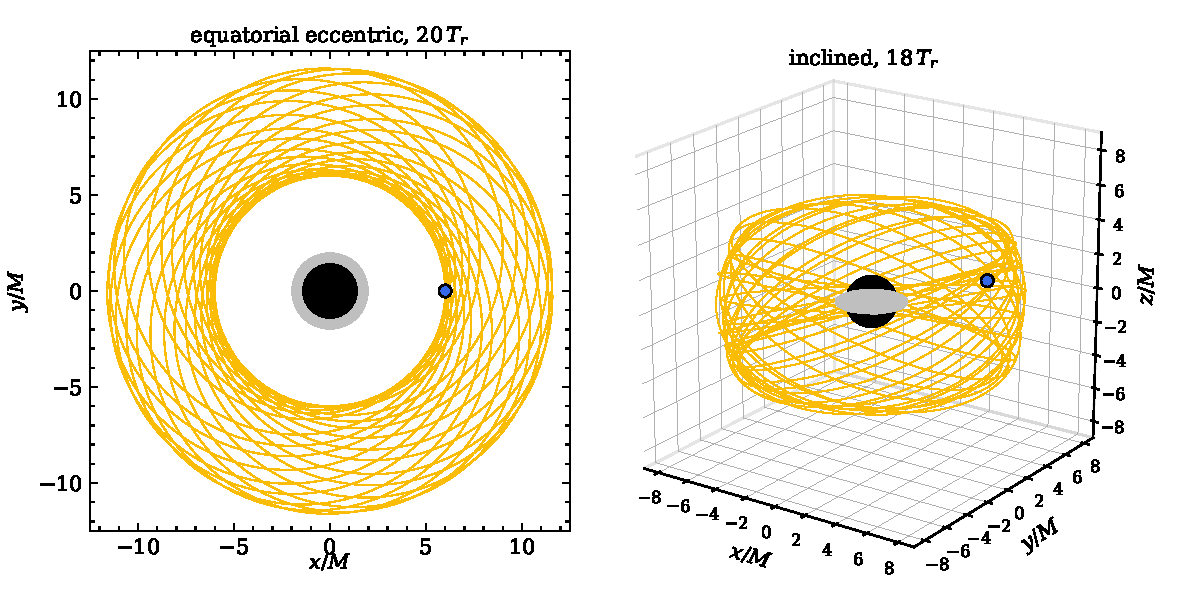
\includegraphics[width=\textwidth]{figures/fig_bl_trajectories.pdf}
\caption{Bound test-particle trajectories around a Kerr black hole ($a = 0.9\,M$) precess coherently and stay confined to their invariant tori. Left: equatorial eccentric orbit; right: inclined three-dimensional orbit [check]. Solid yellow curves show the spacetime Boris pusher in the symmetric gauge on the analytic Boyer--Lindquist metric from initial blue markers outside the black event horizon and gray ergosphere [check].}
\label{fig:orbits}
\end{figure*}

Sending a particle onto a near-capture eccentric trajectory tests whether the implicit midpoint pusher reproduces the strong-field invariant accuracy in Ref.~\cite{Wu:2026nrpic}. In Kerr--Schild coordinates, an inclined passage ($a = 0.9\,M$, $e = 0.99$) grazes the event horizon before returning outward (Fig.~\ref{fig:passage}). Because the midpoint update of Sec.~\ref{sec:pushers} depends solely on the coordinate metric and its spatial derivatives, its discrete trajectory is uniquely fixed. On the analytic spherical Kerr--Schild metric, the implicit midpoint pusher conserves cyclic $L_z$ to rounding error and reproduces all published digits of the maximum relative errors in $\Egeo$ and $Q$ \cite{Wu:2026nrpic}. On the Cartesian Kerr--Schild metric reconstructed via the Hermite weights of Sec.~\ref{sec:reconstruction}, where the grid breaks continuous axisymmetry, it again matches all published digits for $\Egeo$, $L_z$, and $Q$ \cite{Wu:2026nrpic}.

\begin{figure*}[t]
\centering
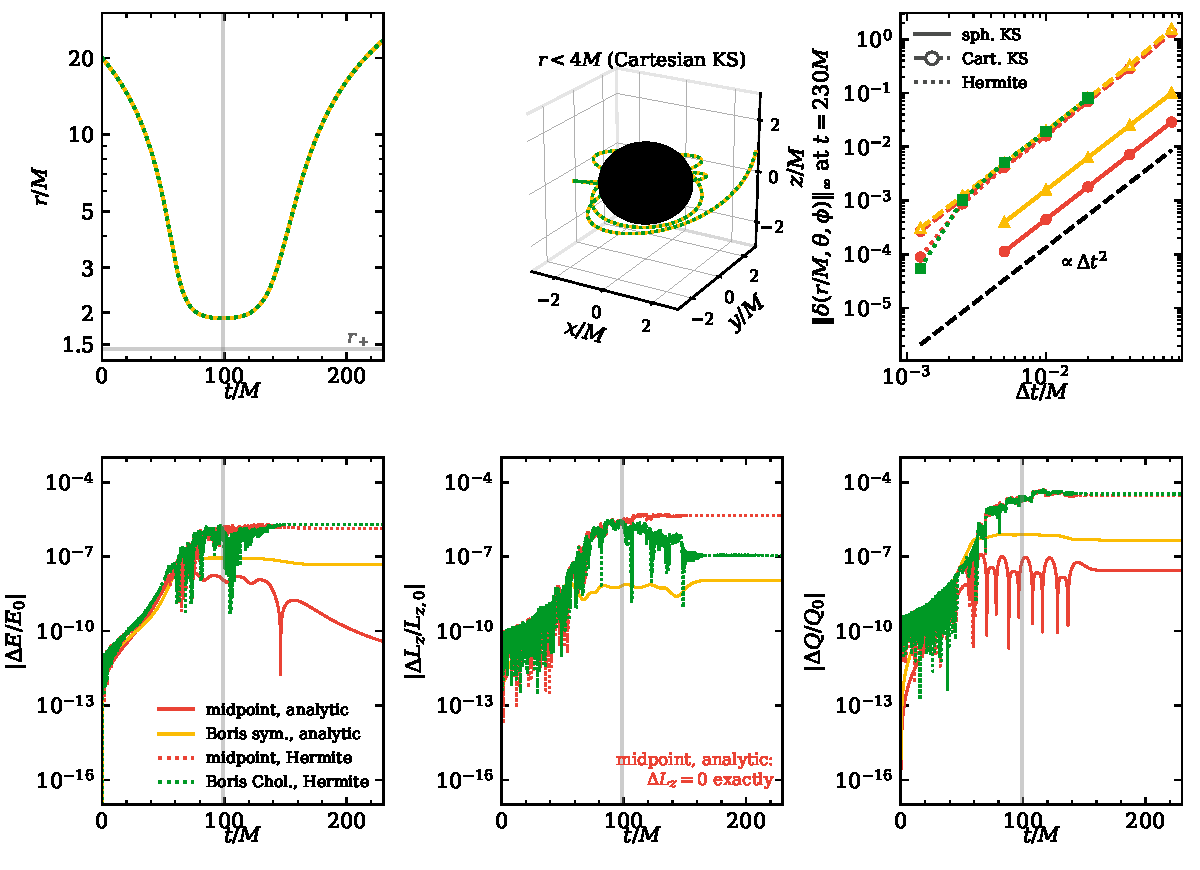
\includegraphics[width=\textwidth]{figures/fig_ks_passage.pdf}
\caption{Both pushers conserve $(\Egeo, L_z, Q)$ through a near-capture Kerr passage ($a = 0.9\,M$, $e = 0.99$), with mesh reconstruction setting the invariant floor and trajectories converging as $\Delta t^2$. Top: radius, near-horizon trajectory, and position error versus $\Delta t$ with a $\Delta t^2$ guide (black dashed); bottom: invariant errors across periapsis (gray) [check]. Colors mark exact or published references (blue), the implicit midpoint pusher (red), and the spacetime Boris pusher in the symmetric (yellow) and Cholesky (green) gauges [check]. Line styles mark analytic spherical (solid), analytic Cartesian (dashed), and mesh-reconstructed (dotted) metrics [check].}
\label{fig:passage}
\end{figure*}

Applying the spacetime Boris pusher to the same passage determines which local orthonormal frames reproduce the published analytic and mesh benchmarks. Off-diagonal spatial metric components in Kerr--Schild coordinates distinguish the symmetric gauge from the Cholesky gauge. Continuous geodesics are frame independent because triad connections in the tetrad equation of motion cancel endpoint projections identically. Over a finite step $\Delta t$, midpoint evaluation of the Boris rotation of Sec.~\ref{sec:pushers} leaves a gauge-dependent second-order error. Reference~\cite{Wu:2026nrpic} leaves the tetrad gauge unspecified. For analytic spherical Kerr--Schild input, the symmetric gauge reproduces all published digits of the $\Egeo$, $L_z$, and $Q$ errors in Ref.~\cite{Wu:2026nrpic} (Fig.~\ref{fig:passage}), while the $(r, \theta, \phi)$ Cholesky gauge gives distinct errors. For mesh-reconstructed Cartesian input, the $(x, y, z)$ Cholesky gauge reproduces all published digits, while the symmetric gauge and permuted Cholesky orderings give distinct values.

Varying the time step $\Delta t$ and cell spacing $h$ independently establishes how trajectory and invariant errors converge across spinning and nonrotating black hole spacetimes. On analytic metrics, position and invariant errors of both pushers and gauges converge at second order in $\Delta t$ across the Kerr orbits and $e = 0.99$ passage (Fig.~\ref{fig:passage}). In the nonrotating limit ($a \to 0$), circular, inclined eccentric, and plunging orbits are tested against exact Schwarzschild solutions (Fig.~\ref{fig:convergence}). Spherical Kerr--Schild circular motion advances linearly in time and azimuth and integrates to rounding error. Cartesian Kerr--Schild circular, eccentric, and horizon-crossing plunging orbits all converge as $\Delta t^2$. Multi-block Cartesian mesh runs at small $\Delta t$ match virtual-lattice runs of spacing $h$ to rounding error across block interfaces. Refining $h$ reduces metric, position, and invariant errors at the third-order rate of cubic Hermite reconstruction for $a = 0.9\,M$ and $a \to 0$ (Fig.~\ref{fig:convergence}).

\begin{figure*}[t]
\centering
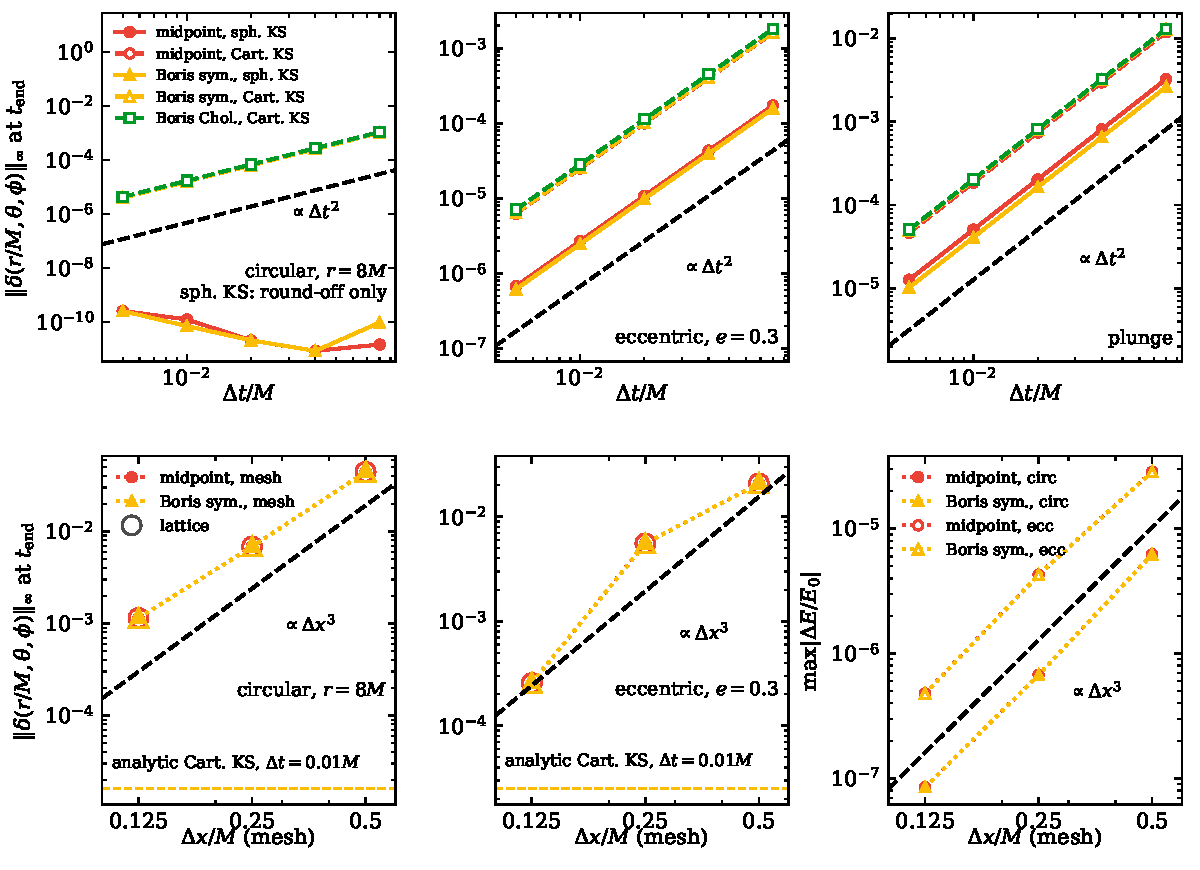
\includegraphics[width=\textwidth]{figures/fig_schwarzschild_convergence.pdf}
\caption{In the nonrotating limit ($a \to 0$), trajectories converge at second order in $\Delta t$ on analytic metrics and at third order in cell spacing $h$ under cubic Hermite reconstruction. Top: position error versus $\Delta t$ for circular, eccentric, and plunging orbits; bottom: position and $\Egeo$ errors versus $h$ on the mesh (dotted) and virtual lattice (open markers) with power-law guides (black dashed) [check]. Curves show the implicit midpoint pusher (red) and the spacetime Boris pusher in the symmetric (yellow) and Cholesky (green) gauges on analytic spherical (solid) and Cartesian (dashed) metrics [check].}
\label{fig:convergence}
\end{figure*}

Comparing mesh-reconstructed trajectories against exact analytic Cartesian trajectories settles whether spatial interpolation or time-stepping truncation governs the Cartesian position error on the $e = 0.99$ passage. Reference~\cite{Wu:2026nrpic} attributes the grid error of both pushers on this passage to spacetime interpolation. Sweeping $\Delta t$ on the analytic Cartesian Kerr--Schild metric alongside the Hermite grid at fixed $h$ separates both effects (Fig.~\ref{fig:passage}). Spatial interpolation dominates the $(\Egeo, L_z, Q)$ errors, which exceed analytic Cartesian values at the published step size and flatten onto an interpolation floor as $\Delta t$ shrinks. Conversely, the analytic Cartesian run without interpolation gives nearly the same final-position error at the published step size as the Hermite grid, and both fall as $\Delta t^2$. Differencing grid and analytic-Cartesian final states at equal $\Delta t$ confirms that pure interpolation shifts the position far less than Cartesian time-stepping until the finest $\Delta t$ tested.

Replacing a single orbit with a cloud of macroparticles tests whether phase mixing on a refined mesh preserves single-particle invariants and analytic trajectories. Gaussian clouds of $N = 10^2$, $10^3$, and $10^4$ bound test particles are initialized around an equatorial circular orbit for $a = 0.9\,M$ and $a \to 0$. Each cloud evolves on both the analytic Cartesian metric and a statically refined octree mesh with passive deposition. Differential orbital shear stretches each cloud into an arc, a trailing spiral, and an azimuthally mixed ring tracked by the deposited energy density $E$ \cite{2008gady.book.....B} (Fig.~\ref{fig:tpcluster}). Vertical epicycles and Kerr nodal precession set the ring thickness. Every macroparticle keeps bounded $(\Egeo, L_z, Q)$ errors free of secular drift, independently of $N$. On the mesh, both pushers give indistinguishable third-order-convergent invariant errors set by Hermite reconstruction and closely match the analytic positions and mixing histories.

\begin{figure*}[t]
\centering
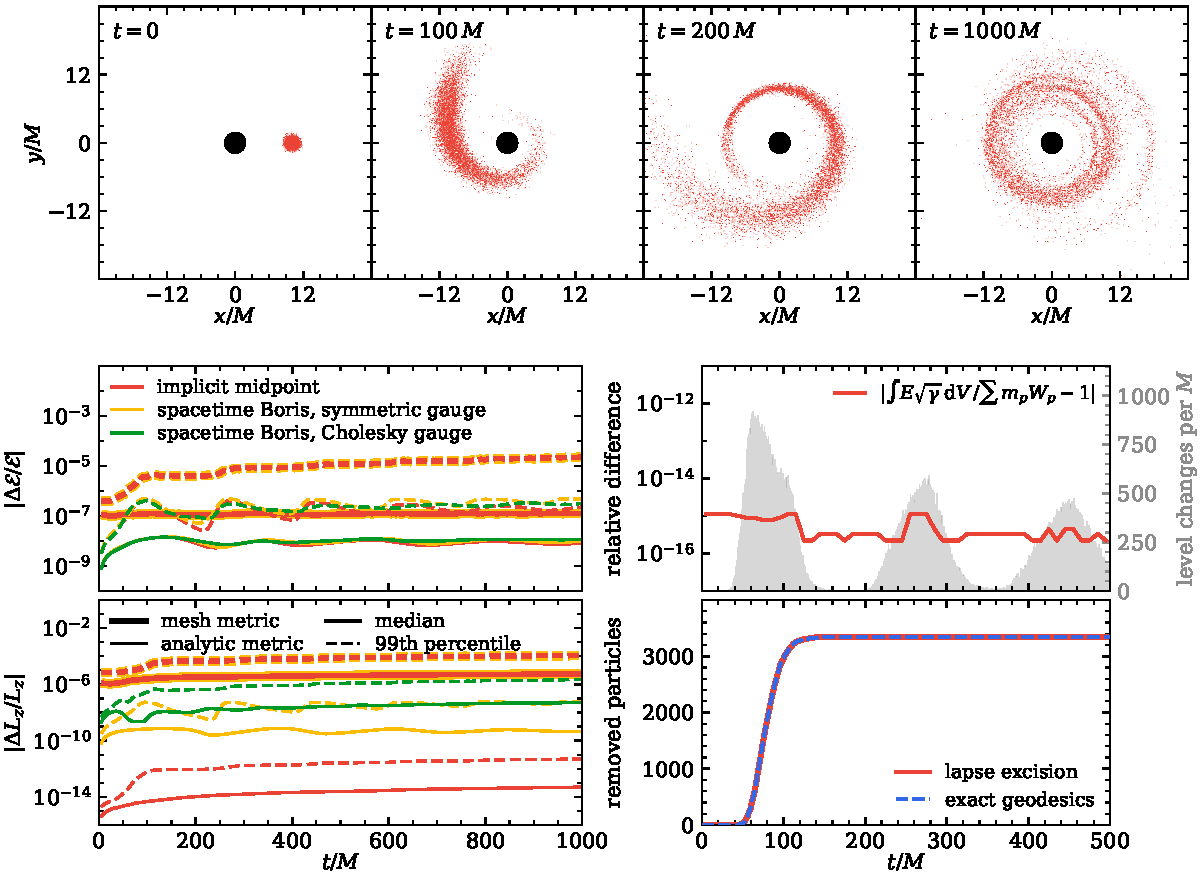
\includegraphics[width=\textwidth]{figures/fig_tp_cluster.pdf}
\caption{A test-particle cluster ($N = 10^4$) around a Kerr black hole ($a = 0.9\,M$) phase-mixes into a ring while conserving single-particle invariants, preserving pre-filter source integrals, and matching exact lapse-excision counts. Panels show phase-mixing snapshots, invariant errors, pre- and post-filter residuals of the conservation identity, and cumulative excised counts [check]. Curves show exact references (blue), the implicit midpoint pusher (red), and the spacetime Boris pusher in the symmetric (yellow) and Cholesky (green) gauges on analytic (solid) and mesh-reconstructed (dotted) metrics [check].}
\label{fig:tpcluster}
\end{figure*}

Accumulating stress-energy from thousands of orbiting macroparticles tests how multi-level deposition and mesh filtering conserve total energy and momentum across refinement boundaries. During phase mixing and infall, macroparticles cross static octree interfaces repeatedly while depositing $(E, S_i, S_{ij})$ in the uncapped limit of the level cap of Sec.~\ref{sec:deposition}. Before filtering, the conservation identity holds to rounding error across all level crossings and excisions whenever clouds lie at least half a cell inside the outer boundary (Fig.~\ref{fig:tpcluster}). For the few large-apocenter particles within half a cell of the outer boundary, cloud weight outside the domain accounts to rounding error for the difference. Subsequent binomial filtering on leaf cells breaks exact conservation at a small level, a limitation of mesh-level smoothing. Averaging $(E, S_i, S_{ij})$ across spatially varying $\sqrt{\gamma}$ and coarse-fine ghost zones shifts proper-volume integrals by a small fraction per boundary-crossing particle (Fig.~\ref{fig:tpcluster}).

Lowering the cluster angular momentum across the capture threshold and varying $N$ test whether lapse excision matches exact geodesic predictions and how sampling noise scales. Plunging-family clusters ($N = 10^4$) for $a = 0.9\,M$ and $a \to 0$ send a large fraction of macroparticles across the event horizon, with exact Kerr effective potentials predicting arrival times at $\aexc$. With both pushers on the mesh, lapse excision matches the predicted removal curve up to a few marginal near-separatrix orbits perturbed across the barrier by interpolation (Fig.~\ref{fig:tpcluster}). Active, excised, and escaped rest masses sum to the initial cluster mass to rounding error. Across independent bound clusters of $N = 10^2$, $10^3$, and $10^4$ macroparticles at fixed total mass, pairwise root-mean-square differences in filtered $E$ fall as $N^{-1/2}$ while diffuse rings remain sampling-noise dominated.

\subsection{Evolving black hole}\label{sec:evolving_black_hole}

Evolving the black hole spacetime dynamically in moving-puncture gauge raises the question of how physical geodesic accuracy can be separated from coordinate drift. A nonrotating vacuum black hole puncture of initial mass $M$ evolves on a statically refined Cartesian mesh under Z4c in moving-puncture gauge (Sec.~\ref{sec:spacetime}) from time-symmetric data with precollapsed lapse. Zero-mass tracers advance on the time-averaged Hermite-reconstructed metric via the implicit midpoint pusher. As $1+\log$ slicing and the Gamma-driver shift relax the slice toward a stationary trumpet \cite{Campanelli:2005dd,Baker:2005vv,Hannam:2008sg}, coordinates drift outward and the coordinate energy $\alpha W - \beta^i u_i$ swings during the gauge transient. Comparison with exact Schwarzschild geodesics therefore uses gauge-independent worldline observables: orbital azimuth, the areal radius $R$ of the sphere of proper area $4\pi R^2$ passing through the particle, and proper time
\begin{equation}\label{eq:particle_proper_time}
\tau(t) = \int_0^t \frac{\alpha}{W}\,\dd t'.
\end{equation}

Tracking radially infalling and plunging tracers tests whether worldlines follow exact strong-field geodesics through the evolving horizon to interior excision. A radial infaller from rest and an inspiraling plunger cross refinement boundaries smoothly, pass the apparent horizon, and undergo lapse excision at $\aexc$ (Fig.~\ref{fig:tracers}). Along radial infall, $R(\tau)$ tracks the exact Schwarzschild cycloid closely outside the horizon, deviating only within a few cells of the puncture where steep gradients limit interpolation of $R$. Along the slower plunge, $R(\tau)$ and azimuth accumulate a small advance relative to the exact geodesic of initial mass $M$. Reintegrating the exact geodesic from the post-transient state with the evolved slice Misner--Sharp mass removes nearly that entire offset (Fig.~\ref{fig:tracers}).

\begin{figure*}[t]
\centering
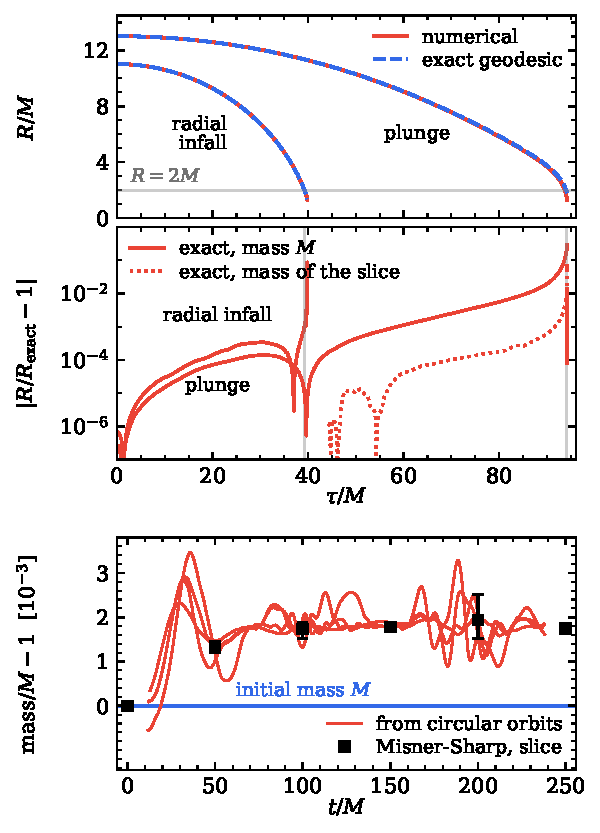
\includegraphics[width=\textwidth]{figures/fig_tracers.pdf}
\caption{Test particles on a numerically evolved moving-puncture black hole spacetime track exact geodesics of the evolved slice in gauge-independent observables. Panels show areal radius $R$ versus proper time $\tau$ with residuals for radial infall and plunge, plus the enclosed mass implied by circular tracers versus slice Misner--Sharp mass [check]. Curves compare exact Schwarzschild geodesics of the initial and evolved masses (blue) with implicit midpoint pusher trajectories on the reconstructed mesh metric (red dotted) [check].}
\label{fig:tracers}
\end{figure*}

Following circular tracers over many dynamical times determines whether their small radial offset reflects pusher error or the evolved black hole slice mass. Equatorial and inclined circular tracers keep planar orbits and conserved angular momentum $L$ while their coordinate radii drift outward and their areal radii $R$ oscillate slightly inside their initial values. Saved spatial slices show that after the early evolution at this resolution, the exterior settles into a uniform Schwarzschild slice whose Misner--Sharp mass is slightly heavier than $M$. Carrying the angular momentum of mass $M$, each tracer starts at the apocenter of a mildly eccentric orbit of that heavier black hole, whose geodesics reproduce the $R(\tau)$ oscillations. In Schwarzschild geometry, areal radius $R$, angular momentum $L$, and radial acceleration imply an enclosed mass
\begin{equation}\label{eq:implied_mass}
M_{\rm eff} = \frac{L^2/R - R^2\,\dd^2 R/\dd\tau^2}{1 + 3L^2/R^2}.
\end{equation}
Across all orbital radii and inclinations, $M_{\rm eff}$ agrees with the slice Misner--Sharp mass (Fig.~\ref{fig:tracers}). Extending these gauge-independent tracer tests to an inspiraling and merging binary black hole in moving-puncture gauge is in progress [pending].
}{}
\IfFileExists{sections/self_gravity.tex}{\section{Self-gravitating matter}\label{sec:selfgravity}

Coupled Einstein-Vlasov dynamics begins once macroparticles carry finite rest mass $m_p$ and feed their deposited sources $(E, S_i, S_{ij})$ back into the spacetime evolution. Collective gravitational wells then form, oscillate, disperse, or collapse into black holes from the matter distribution itself, closing the particle-mesh cycle of Sec.~\ref{sec:method}. Whereas Ref.~\cite{Wu:2026nrpic} evolves its main self-gravitating benchmarks with about $10^6$ to $5 \times 10^6$ macroparticles on large machines, every run here uses at most ten thousand ($N \le 10^4$) on one graphics card. Quantities independent of $N$, such as continuum equilibrium sequences and analytic collapse bounds, test the coupled solver at full precision. Phenomena sensitive to discrete sampling---initial lattices, multi-pass filtering, refinement under diffuse matter, and cluster holding---isolate what changes at $N \le 10^4$, with scenario parameters listed in the appendix.

\subsection{Dust collapse}\label{sec:dust}

Spherical collapse of cold, pressureless matter from rest tests the coupled solver from smooth initial curvature through black hole formation against an exact solution \cite{Oppenheimer:1939ue}. A homogeneous dust ball of initial areal radius $R_0 = 5\,M$, ADM mass $M$, and uniform density $E_0 = \rho_0 = 3M/(4\pi R_0^3)$ starts at rest on a conformally flat slice \cite{Petrich:1985jko,Staley:2011ss,Wu:2026nrpic}. At $t = 0$, momenta $u_{i,p}$, extrinsic curvature $K_{ij}$, and shift $\beta^i$ vanish, $\alpha = 1$, and interior and exterior $\psi$ join smoothly at isotropic radius $\rbar_0$. Nearly $10^4$ macroparticles occupy a cubic lattice of spacing $h$ inside $\rbar_0$ and evolve with dynamic refinement, one plain binomial filter pass, and lapse excision. Along free-falling worldlines parameterized by $\varphi \in [0, \pi)$, shell areal radius $R$, central proper time $\tau_c$, and interior density $E$ follow the cycloid \cite{Oppenheimer:1939ue},
\begin{align}\label{eq:cycloid}
R(\varphi) &= \frac{R_0}{2}(1 + \cos\varphi), \qquad
\tau_c(\varphi) = \sqrt{\frac{R_0^3}{8M}}\,(\varphi + \sin\varphi), \nonumber\\
E(\varphi) &= E_0\!\left(\frac{R_0}{R(\varphi)}\right)^3.
\end{align}
Because $1+\log$ slicing ties $\partial_t\alpha$ to local volume contraction, $\alpha_c$ tracks central compression directly. From unit initial lapse without shift advection, local integration inside the homogeneous core gives an analytic lower bound on $\alpha_c$, the lapse bound \cite{Staley:2011ss},
\begin{equation}\label{eq:lapse_bound}
\alpha_{\rm bound}(\tau_c) = 1 + 6\ln\!\left(\frac{R(\tau_c)}{R_0}\right).
\end{equation}
The surface density jump launches an inward gauge wave in the slicing coordinate $\alpha$. Until that gauge wave reaches the origin, causal isolation keeps $\alpha_c(\tau_c)$ on the lapse bound while the dust falls freely.

Central infall and black hole formation are expected to match continuum Oppenheimer--Snyder collapse despite the discrete particle representation. In the simulation (Fig.~\ref{fig:dust}, top left), $\alpha_c(\tau_c)$ tracks the lapse bound closely during causal isolation and departs smoothly once the surface gauge wave arrives, matching Ref.~\cite{Wu:2026nrpic} and continuum runs \cite{Staley:2011ss}. Until the center refines to $\Delta x = h/4$, the central density $E_c(\tau_c)$ likewise follows the cycloid closely (Fig.~\ref{fig:dust}, top right, red curve). At $\Delta x = h/4$, fine cells outnumber nearby particles and leave part of the central probe empty, dropping $E_c$ below the cycloid until infall concentrates particles inward. As strong-field curvature grows, $1+\log$ slicing drives $\alpha_c$ toward zero and an apparent horizon forms around the matter (Fig.~\ref{fig:dust}, bottom left). Shortly afterward, interior $\alpha$ drops below $\aexc$ and lapse excision removes every macroparticle. Meanwhile, the Hamiltonian constraint norm $\|\Ham\|$ (Sec.~\ref{sec:spacetime}; Table~\ref{tab:outcomes_dust}) peaks and damps across the vacuum ringdown (Fig.~\ref{fig:dust}, bottom right).

\begin{figure*}[t]
\centering
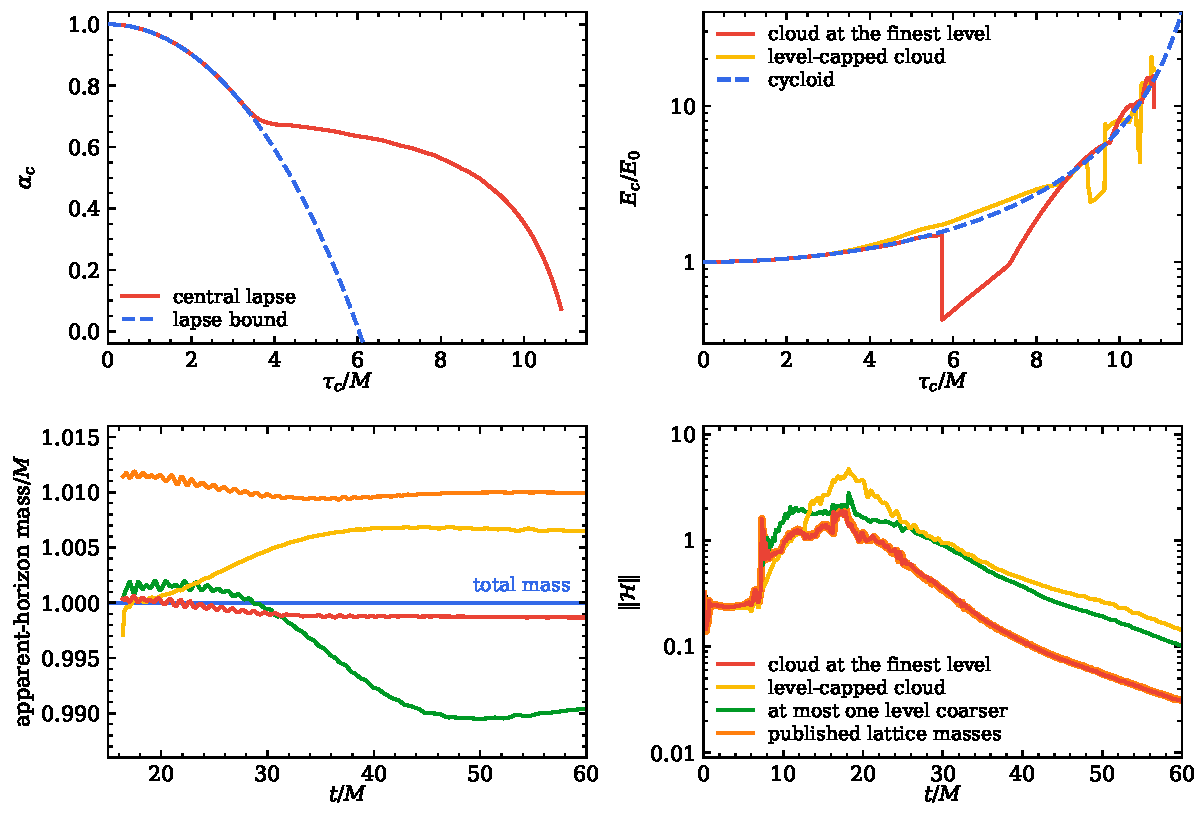
\includegraphics[width=\textwidth]{figures/fig_dust.pdf}
\caption{Gravitational collapse of a pressureless dust ball ($R_0 = 5\,M$, nearly $10^4$ macroparticles) to a black hole on an adaptive mesh. Top left: central lapse $\alpha_c$ versus central proper time $\tau_c$ (red) and the analytic lapse bound (blue dashed). Top right: central energy density $E_c/E_0$ and the cycloid (blue dashed) before central excision. Bottom: apparent-horizon mass with total mass $M$ (blue), and Hamiltonian constraint norm $\|\Ham\|$. Curves show finest-level clouds with surface-corrected (red) or published (orange, bottom) lattice masses, and level-capped clouds with unlimited (yellow) or one-level (green, bottom) coarsening.}
\label{fig:dust}
\end{figure*}

At $N \lesssim 10^4$, discrete lattice initialization must match the particle rest-mass sum to the continuum rest mass $M_0$ of the initial slice. With published lattice masses \cite{Wu:2026nrpic}, each site inside $\rbar_0$ carries rest mass $m_p = \rho_0 \psi(\bm{x}_p)^6 h^3$, the local proper rest-mass density times the cell volume. Those masses were first assumed to yield a black hole of mass $M$ here, as at $N \sim 10^6$ where surface count offsets vanish. At $N \lesssim 10^4$, however, the count of lattice sites inside a sphere differs from its volume in cells. On the lattice of Table~\ref{tab:setups} ($26$ cells across $2\rbar_0$), that count exceeds the cell volume and leaves $\sum_p m_p$ above $M_0$ (Table~\ref{tab:outcomes_dust}). Runs with published lattice masses kept the interior density exact, so $\alpha_c$ and $E_c$ still matched the surface-corrected collapse. Their apparent-horizon mass $M_{\rm AH}$, however, formed visibly above $M$ (Fig.~\ref{fig:dust}, bottom left, orange curve; Table~\ref{tab:outcomes_dust}). Radial profiles of the slice Misner--Sharp mass $M_{\rm MS}$ traced this excess to a mass shell leaving the boundary at $t = 0$ at light speed, outside which $M_{\rm MS}$ equaled $M$. The surface correction of Sec.~\ref{sec:numerical_methods} rescales $m_p$ in the outermost lattice layer of width $h$ so $\sum_p m_p = M_0$ with interior masses unchanged. With surface-corrected lattice masses, $M_{\rm AH}$ at formation matches $M$ to within the accuracy of the mass measure and drifts downward only slightly afterward (Fig.~\ref{fig:dust}, bottom left, red curve; Table~\ref{tab:outcomes_dust}).

Reliable horizon masses after collapse require checking the apparent-horizon finder on a vacuum black hole of known mass $M$ without matter or excision. In initial collapse tests, AthenaK's distributed pseudospectral flow finder \cite{Gundlach:1997us,2026ApJS..283...27S,Zhu:2024utz} returned horizon masses visibly below $M$. A first reading, that the flow iteration stopped too early, was ruled out on an evolved vacuum puncture of mass $M$ (Sec.~\ref{sec:evolving_black_hole}) when a much tighter stopping rule left the deficit unchanged. Across three cell spacings on that puncture, AthenaK's distributed finder reported masses well below $M$, with a deficit that is nonmonotonic in cell size (Fig.~\ref{fig:horizoncheck}, top panel, solid curves; Table~\ref{tab:outcomes}). On the same slices, we evaluated the slice Misner--Sharp mass $M_{\rm MS}$, the enclosed mass from slice geometry alone (Sec.~\ref{sec:numerical_methods}; Fig.~\ref{fig:horizoncheck}, open circles). Whereas $M_{\rm MS}$ fell short of $M$ on the coarsest mesh, it matched $M$ on the two finer meshes where the black hole is resolved (Table~\ref{tab:outcomes}). On those two resolved meshes, the evolved spacetime carried the mass $M$ and the deficit belonged to the finder. Inspection of the finder showed that it interpolates metric derivatives stored on active cells, whose ghost zones remain unfilled across block faces (Secs.~\ref{sec:numerical_methods} and \ref{sec:assembly}). Relative to $M_{\rm MS}$, the finder deficit is largest on the finest mesh, where blocks are narrowest and more block faces cut the origin-centered horizon. Direct differentiation of the ghost-filled Lagrange metric interpolant on the trial surface eliminates those block-face errors and restores spherical zero-expansion horizons. At the two finer cell sizes, the corrected apparent-horizon mass $M_{\rm AH}$ matches $M_{\rm MS}$ closely on saved slices and in a live run (Fig.~\ref{fig:horizoncheck}, dashed curve and diamonds; Table~\ref{tab:outcomes}).

\begin{figure}[t]
\centering
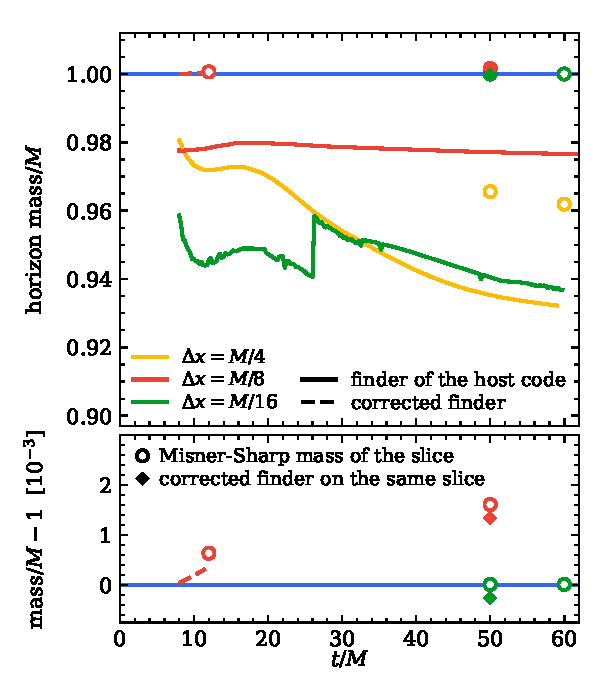
\includegraphics[width=\columnwidth]{figures/fig_horizon_check.pdf}
\caption{Apparent-horizon mass of a vacuum black hole of mass $M$ (blue) at three cell spacings (colors). Solid curves show the host code's finder, and the dashed curve differentiates the metric interpolant. Circles show the slice Misner--Sharp mass and diamonds the corrected finder on the same slices (enlarged below).}
\label{fig:horizoncheck}
\end{figure}

Level-capped deposition (Sec.~\ref{sec:deposition}) sets $\lcap$ from local particle density so sparse refined regions deposit onto virtual cloud cells of width near the initial particle spacing $h$. On the surface-corrected lattice, an unlimited cap removes the $\|\Ham\|$ jump when the center refines to $\Delta x = h/4$ (Fig.~\ref{fig:dust}, bottom right; Table~\ref{tab:outcomes_dust}). Although innermost particle radii stay identical across the runs, the central-density reading $E_c(\tau_c)$ then sits above the cycloid (Fig.~\ref{fig:dust}, top right, yellow curve). That excess arises because the contracting particle lattice beats against virtual cloud cells of nearly equal spacing $h$ at the center. Stored particles from the finest-level run reproduce these $E_c$ readings when redeposited onto width-$h$ clouds. Near the forming black hole, the unlimited cap raises $\|\Ham\|$ and drives $M_{\rm AH}$ above $M$ after excision. A one-level coarsening cap raises $E_c$ further (Table~\ref{tab:outcomes_dust}), elevates $\|\Ham\|$, and shifts $M_{\rm AH}$ to about one percent below $M$ (Fig.~\ref{fig:dust}, bottom panels, green curves).

Randomly sampled dust controls test finest-level against level-capped clouds at two refinement depths (Tables~\ref{tab:setups} and \ref{tab:outcomes_dust}). At full depth ($\Delta x = h/8$) under plain or compensated filtering, finest-level clouds follow sampling noise past the block limit before an apparent horizon forms. At that depth under either filter, level-capped clouds keep refinement bounded through black hole formation with $M_{\rm AH}$ within a few tenths of a percent of $M$. One refinement level shallower ($\Delta x = h/4$) with compensated filtering, both finest-level and level-capped runs complete on the same random sample. In that paired comparison without a lattice, level-capped clouds still raise $\|\Ham\|$ after black hole formation and shift $M_{\rm AH}$ lower by a few tenths of a percent (Table~\ref{tab:outcomes_dust}). That paired run refuted an initial explanation attributing the coarser-cloud disturbance to the lattice beat alone. Coarser clouds raise constraint residuals near a forming black hole and shift $M_{\rm AH}$ by a few tenths of a percent, more on a lattice, yet bound deep refinement on random samples. Finest-level clouds are more accurate where refinement stays bounded and are used for every production collapse run, while the level-capped runs serve as controls.

\subsection{Prolate collapse}\label{sec:prolate}

Cold prolate collapse from rest tests the coupled solver in three dimensions beyond spherical symmetry. Transverse infall focuses collisionless matter onto the symmetry axis into a caustic before any apparent horizon forms. Early axisymmetric simulations found rapidly growing curvature ahead of any apparent horizon \cite{Shapiro:1991zza}. Analytic examples showed that spatial slices of a black hole spacetime can miss trapped surfaces \cite{Wald:1991zz}. Three-dimensional particle runs later found resolution-dependent curvature peaks inside the spindle for this model \cite{Yoo:2016kzu}. Generalized-harmonic evolutions then followed collapse past the caustic to black hole formation \cite{East:2019bwu}. Particle-in-cell Z4c runs likewise formed an apparent horizon after the caustic \cite{Wu:2026nrpic}. A homogeneous spheroid of mass $M$ and eccentricity $e = 0.9$ starts from rest with $N = 10^4$ symmetric equal-mass macroparticles (Appendix~\ref{app:sampling}) on an adaptive mesh (Table~\ref{tab:setups}).

Radial infall contracts the spheroid into a thin spindle (Fig.~\ref{fig:prolate}, top row, at saved snapshots nearest the published times \cite{Wu:2026nrpic}). At $N = 10^4$ this spindle is an axial chain of separate condensations (Fig.~\ref{fig:prolate}, third panel). Equatorial reflection symmetry of the sample places two mirror-image maxima of the Kretschmann scalar $I$ (Sec.~\ref{sec:numerical_methods}) inside the matter on the axis, first near the ends \cite{Wu:2026nrpic}. Those maxima move inward in steps as peak $I$ jumps between condensations (Fig.~\ref{fig:prolate}, bottom left). Peak $I$ depends on cell spacing \cite{Wu:2026nrpic}, with an upward jump in Fig.~\ref{fig:prolate} when the finest mesh levels appear. With grid curvature finite throughout focusing, the run continues through the stage of largest curvature. An apparent horizon first forms at the time shown in Ref.~\cite{Wu:2026nrpic}, with spindle tips extending past its poles (Fig.~\ref{fig:prolate}). Lapse excision below $\aexc$ then removes all $10^4$ macroparticles as those tips fall into the black hole.

\begin{figure*}[t]
\centering
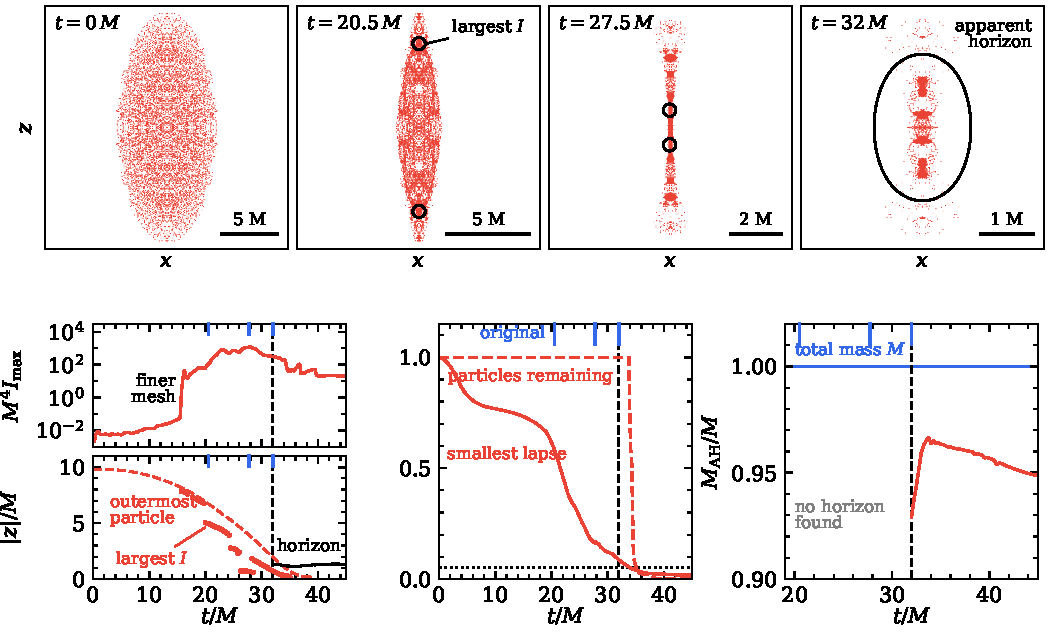
\includegraphics[width=\textwidth]{figures/fig_prolate.pdf}
\caption{The cold prolate spheroid ($e = 0.9$, $N = 10^4$) collapses into a segmented spindle whose two axial curvature maxima step inward before an apparent horizon forms. Top: $x$--$z$ macroparticles, maxima of the Kretschmann scalar $I$ (circles), and first apparent horizon (black). Bottom left: peak $I$, plus axial $|z|$ of that peak (red), outermost macroparticle (red dashed), and horizon (black). Bottom middle and right: smallest lapse with $\aexc$ (dotted) and surviving fraction (red dashed), and $M_{\rm AH}$ with $M$ (blue). Vertical dashed lines mark first horizon; blue ticks mark snapshot times \cite{Wu:2026nrpic}.}
\label{fig:prolate}
\end{figure*}

The apparent-horizon mass $M_{\rm AH}$ (Sec.~\ref{sec:numerical_methods}) peaks about five percent below $M$ after polar infall (Fig.~\ref{fig:prolate}, bottom right; Table~\ref{tab:outcomes_prolate}). That apparent-horizon mass continues to fall at the end of the run. Reference~\cite{Wu:2026nrpic} states no apparent-horizon mass for this test. The slice Misner--Sharp mass $M_{\rm MS}$ (Sec.~\ref{sec:numerical_methods}) on the final slice agrees with the finder at the apparent horizon within its angular spread (Table~\ref{tab:outcomes_prolate}). The same profile $M_{\rm MS}$ recovers the total mass $M$ at large radius. The remaining five to eight percent of $M$ after lapse excision reside in gravitational fields outside the black hole (Table~\ref{tab:outcomes_prolate}). Outside the black hole, $M_{\rm MS}(R) - M_{\rm AH}$ sums radiated gravitational-wave energy and geometric mass from constraint violations without separating them. The Hamiltonian constraint norm $\|\Ham\|$ peaks at largest curvature about three times above its lattice dust peak (Sec.~\ref{sec:dust}; Table~\ref{tab:outcomes_prolate}). A spherical control with a random sample and the same filter loses only a few tenths of a percent of $M$, so random sampling alone does not explain this deficit. How the deficit of the prolate collapse splits between particle number and cell size at its caustic stage is not determined. Dynamic refinement (Sec.~\ref{sec:amr}) with halved finest cells exceeds the block memory of one graphics card, which sets our finest grid.

On the prolate sample at $\Delta x = M/32$, four binomial passes with compensation (Sec.~\ref{sec:deposition}) remove only the early noise-driven refinement. Curvature along the collapsing spindle itself still drives the block count past the memory limit before an apparent horizon forms. The production run stays bounded because its refinement depth is limited by one level ($\Delta x = M/16$) alongside that compensated filter (Table~\ref{tab:setups}).

\subsection{Relativistic clusters}\label{sec:clusters}

Warm collisionless star clusters in equilibrium balance collective gravity through velocity dispersion. Their evolution tests phase-space conservation alongside general-relativistic radial stability \cite{1968ApJ...154..251I,1980ApJ...238.1101I,1985ApJ...298...34S,1985ApJ...298...58S}. As in Shapiro and Teukolsky \cite{1985ApJ...298...34S,1985ApJ...298...58S} and Ref.~\cite{Wu:2026nrpic}, static, spherically symmetric, isotropic monoenergetic (single-energy) clusters populate one Killing energy $\Egeo = \alpha W = \alpha_{\rm s}$. Here $\alpha_{\rm s}$ is the lapse at the cluster surface, where particle speed vanishes ($W = 1$). Radial integration of the Einstein-Vlasov equilibrium relations---the structure equations---yields a one-parameter sequence labeled by $y_c \in (0, 1)$, with gravitational binding energy $E_b$,
\begin{equation}\label{eq:cluster_sequence}
y_c = \left(\frac{\alpha_{c,\rm eq}}{\alpha_{\rm s}}\right)^2, \qquad
E_b = M_0 - M.
\end{equation}
In this sequence, $\alpha_{c,\rm eq}$ is the equilibrium central lapse, $z_c = \alpha_{c,\rm eq}^{-1} - 1$ is the central redshift, $M_0$ is total rest mass, and $M$ is ADM mass \cite{1985ApJ...298...34S,Andreasson:2011ng}. From diffuse, nearly Newtonian clusters ($y_c \to 1$, low $z_c$) to compact, relativistic cores (smaller $y_c$, high $z_c$), $E_b/M_0$ rises to one maximum along the sequence. At still smaller $y_c$, $E_b$ decreases and turns negative ($M > M_0$). Like the turning point of fluid stars \cite{Chandrasekhar:1964zz,Friedman:1988er}, that binding-energy maximum separates stable clusters at larger $y_c$ from unstable clusters at smaller $y_c$ \cite{1980ApJ...238.1101I,1985ApJ...298...58S,Wu:2026nrpic}. Perturbed clusters on the high-$y_c$ branch hold together, whereas clusters past the maximum collapse or expand. Each unit-mass cluster draws up to $10^4$ equal-mass macroparticles with zero net momentum (Sec.~\ref{sec:numerical_methods}). Static meshes evolve the two loosest models and adaptive meshes evolve the kicked compact ones, with all meshes and particle numbers in Table~\ref{tab:setups}.

Multi-pass grid filtering suppresses discrete source fluctuations at $N = 10^4$, yet uncompensated smoothing biases self-gravitating equilibria outward. An unperturbed cluster on the stable branch ($y_c = 0.819$) was expected to stay near equilibrium with minor oscillations, as for the kicked model in Ref.~\cite{Wu:2026nrpic}. With four plain binomial passes, the cluster instead expanded by a visible fraction of its radius and dropped in central density before rebounding. Over that bounce, $\alpha_c$ rose well above $\alpha_{c,\rm eq}$ (Fig.~\ref{fig:filter}, left panel, solid curves; Table~\ref{tab:outcomes_clusters}). A first reading, that discrete sampling noise drove this excursion, was ruled out when three independent $10^4$-particle samples traced the identical bounce up to a tiny ripple (Fig.~\ref{fig:filter}, left panel). Sweeps across zero, two, and four plain passes on one sample showed that the initial lapse rise grows systematically with pass count $n_{\rm f}$ (Fig.~\ref{fig:filter}, middle panel). Each plain binomial pass widens every cloud's second moment, which acts as a gravitational softening over the filter scale \cite{2008gady.book.....B} (Sec.~\ref{sec:deposition}). Plain passes also lower the proper-volume integral of $E$ slightly across nonuniform $\sqrt{\gamma}$. Because particle velocities match the unsoftened equilibrium, that shallower smoothed potential lets the cluster expand and recontract. The compensation pass of Sec.~\ref{sec:deposition} \cite{1991ppcs.book.....B} cancels that second-moment softening and preserves the proper-volume energy integral. It removes the bounce across two and four passes and leaves $\alpha_c(t)$ insensitive to $n_{\rm f}$ (Fig.~\ref{fig:filter}, dashed curves). Unfiltered evolution ($n_{\rm f} = 0$) also avoids the bounce, yet leaves $\|\Ham\|$ much higher (Table~\ref{tab:outcomes_clusters}) and causes $\alpha_c$ to wander downward later (Fig.~\ref{fig:filter}, middle panel). All cluster runs below therefore combine four binomial passes with compensation.

\begin{figure*}[t]
\centering
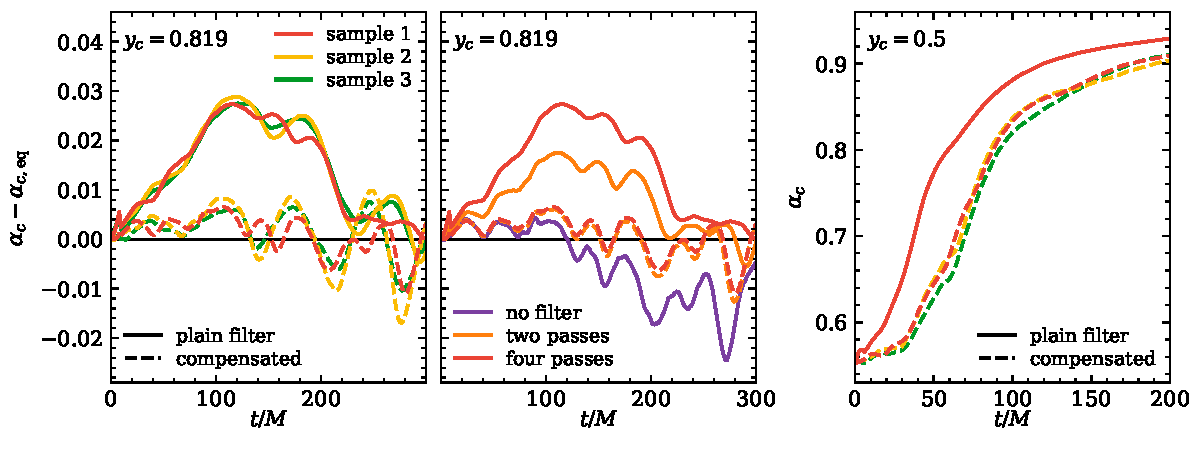
\includegraphics[width=\textwidth]{figures/fig_filter.pdf}
\caption{Source filtering and radial motion of monoenergetic clusters with $N = 10^4$ macroparticles. Left: central-lapse offset $\alpha_c - \alpha_{c,\rm eq}$ from equilibrium (black line) for the stable model $y_c = 0.819$ across three samples (colors), comparing four plain binomial passes (solid) with compensated filtering (dashed). Middle: one sample with zero, two, and four filter passes (colors), plain (solid) and compensated (dashed). Right: central lapse $\alpha_c$ of the unperturbed unstable model $y_c = 0.5$, encoded as on the left.}
\label{fig:filter}
\end{figure*}

Dynamically stable clusters on the high-$y_c$ side of the binding-energy maximum are expected to remain bound and oscillate stably under small radial perturbations. As in Ref.~\cite{Wu:2026nrpic}, we apply a one-percent inward velocity kick to the stable models $y_c = 0.900$ and $y_c = 0.819$ at $N = 10^4$ (Fig.~\ref{fig:clusters}, first two columns). Over several crossing times, both clusters retain every macroparticle and stay centered near the origin, as in Ref.~\cite{Wu:2026nrpic}. Rest-mass radii stay within a narrow band for $y_c = 0.900$ and undergo bounded radial swings in the inner shells of $y_c = 0.819$ (Fig.~\ref{fig:clusters}, top left). Because its potential is shallower, the looser model $y_c = 0.900$ shows much smaller variations in $\alpha_c$ (Table~\ref{tab:outcomes_clusters}) and mean Lorentz factor than $y_c = 0.819$.

\begin{figure*}[t]
\centering
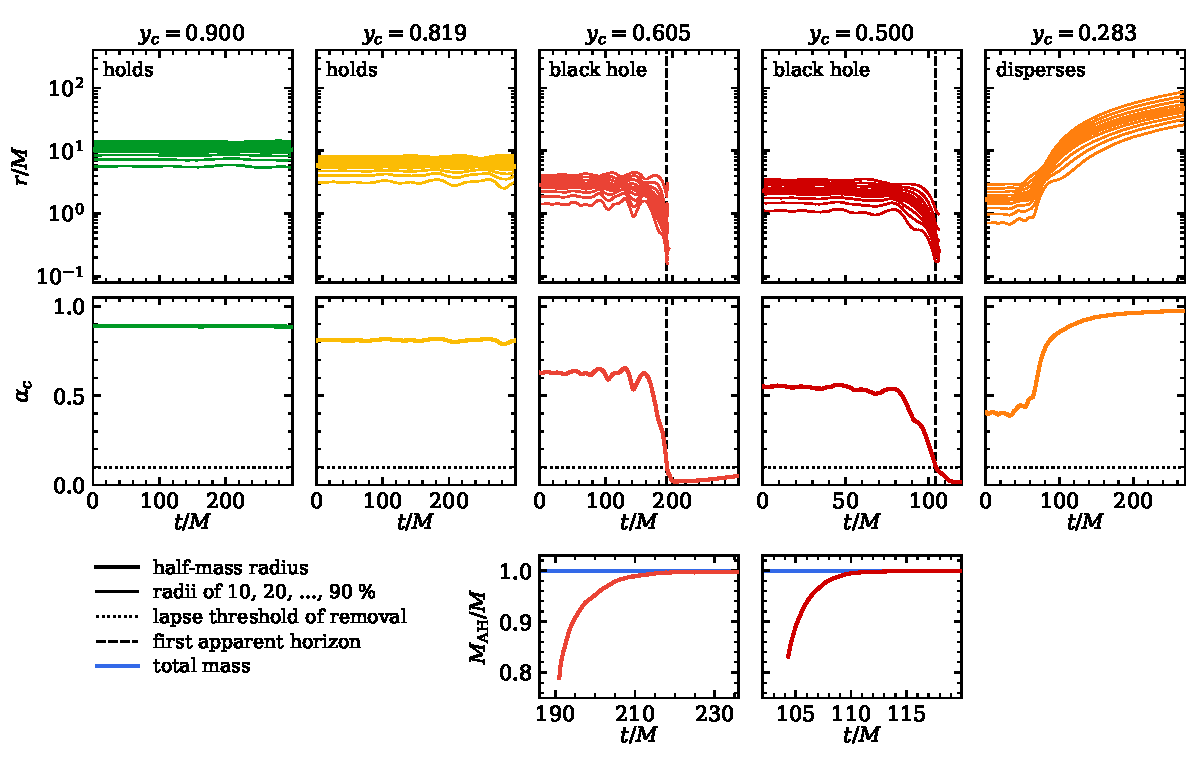
\includegraphics[width=\textwidth]{figures/fig_clusters.pdf}
\caption{Five monoenergetic clusters ($N = 10^4$) with an inward velocity kick, ordered from least compact (left) to most compact (right). Models $y_c = 0.900$ and $0.819$ hold, $0.605$ and $0.500$ form black holes, and the unbound model $0.283$ disperses. Top: coordinate radii enclosing tenths of remaining rest mass (half-mass thicker) while at least half remains. Middle: central lapse $\alpha_c$ with excision threshold $\aexc$ (dotted) and first apparent horizon (dashed, also top). Bottom: apparent-horizon mass $M_{\rm AH}$ and total mass $M$ (blue).}
\label{fig:clusters}
\end{figure*}

Closer inspection of the stable model $y_c = 0.819$ reveals a coherent radial oscillation of its core that grows before saturating at late times. With filter softening removed, an unperturbed equilibrium was expected to hold a steady central lapse $\alpha_c = \alpha_{c,\rm eq}$. Instead, $\alpha_c$ oscillates at a period close to the radial period of a particle in the core (Fig.~\ref{fig:oscillation}, top panel; Table~\ref{tab:outcomes_clusters}), while the outer shells stay within a few percent of their initial radii over the first three hundred $M$ and move more afterward. Because a nearly uniform core creates an almost harmonic potential with a shared radial period, collective core motion resists phase mixing \cite{2008gady.book.....B}. Over the first several periods the swing grows steadily, so a long continuation tested unbounded instability against saturation. In that extended run, growth halts after several cycles and the swing stays bounded at a small fraction of $\alpha_{c,\rm eq}$ with all $10^4$ particles retained (Fig.~\ref{fig:oscillation}, top panel). A first reading, that intermediate-wavenumber sampling noise passed by the compensated filter excited this mode, was ruled out by three stratified samples (Fig.~\ref{fig:oscillation}, top panel) and a Monte Carlo sample. All samples share the same period, phase, and growth. Inward-kicked runs at $N = 10^3$ and $10^4$ likewise show matching early swings without $N^{-1/2}$ amplification (Fig.~\ref{fig:oscillation}, bottom left; Table~\ref{tab:outcomes_clusters}).

Further controls on the first sample tested whether time-stepping lag, constraint handling, cloud width, or cell spacing drives this core oscillation (Fig.~\ref{fig:oscillation}, bottom middle and right; Table~\ref{tab:setups}). Frozen sources across $\Delta t$ could lag particle motion, yet a halved step $\Delta t/2$ leaves $\alpha_c(t)$ unchanged. Feedback from constraint damping or advected constraint residuals was tested across raised and zero $\kappa_1$ and with parabolic relaxation of the Hamiltonian constraint (Sec.~\ref{sec:spacetime}). Although those settings alter $\|\Ham\|$ substantially, all three reproduce $\alpha_c(t)$ to a tiny fraction of the swing (Fig.~\ref{fig:oscillation}, bottom right; Table~\ref{tab:outcomes_clusters}). An extended compensation weight $c$ that also cancels cloud width trims the slow excursion slightly while leaving the oscillation intact (Fig.~\ref{fig:oscillation}, bottom middle; Table~\ref{tab:outcomes_clusters}). A control with halved cell spacing over the cluster (Table~\ref{tab:setups}) leaves the first $\alpha_c$ maximum unchanged, gives an equal or slightly larger growth rate, and drifts further in mean lapse. That control refutes a second-order cell-size origin for the oscillation. In the sequence figure of Ref.~\cite{Wu:2026nrpic}, the full-range lapse axis is too coarse to resolve a swing of $0.01$ in $y_c = 0.819$. By contrast, the narrower-axis figure for the perturbed near-critical cluster in Ref.~\cite{Wu:2026nrpic} at $N = 10^6$ displays the same growth, saturation, and decay at the core period. What sets the small common initial offset from which the unperturbed oscillation starts here is not determined.

\begin{figure*}[t]
\centering
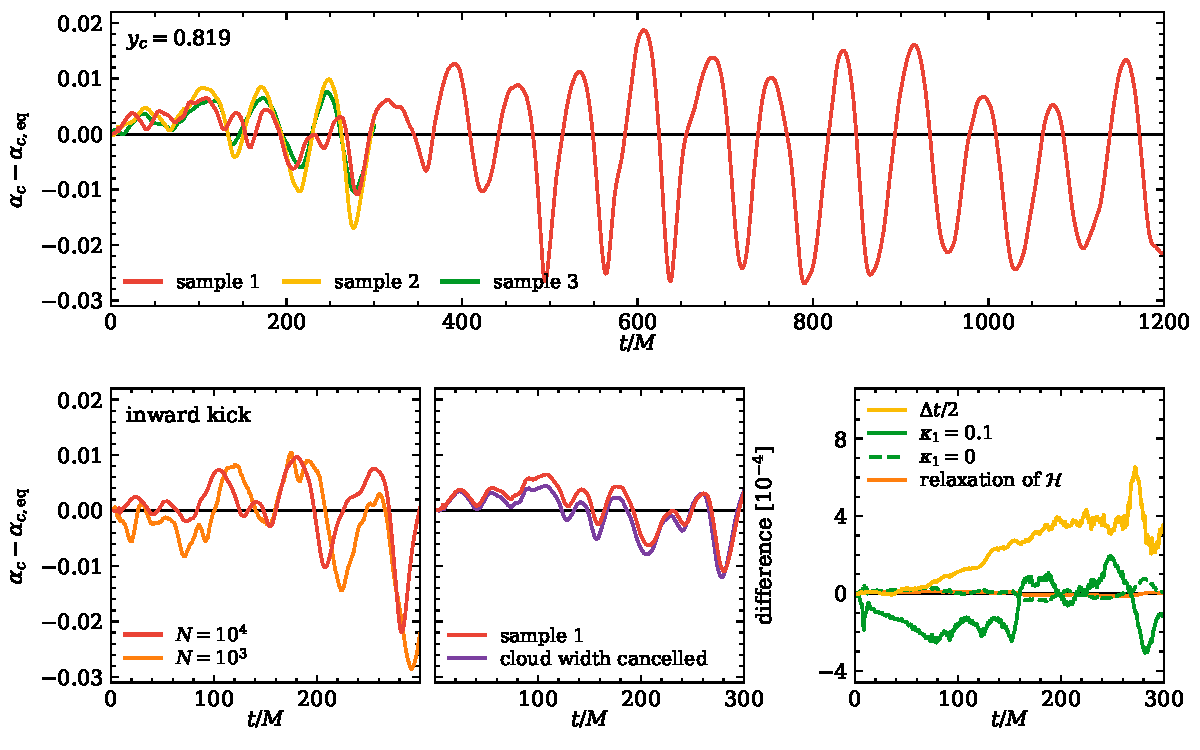
\includegraphics[width=\textwidth]{figures/fig_oscillation.pdf}
\caption{Core oscillation of the stable cluster $y_c = 0.819$ in central-lapse offset $\alpha_c - \alpha_{c,\rm eq}$ from equilibrium (black lines). Top: three unperturbed samples at $N = 10^4$ (colors), with sample 1 continued to saturation. Bottom left: inward-kicked runs at $N = 10^4$ and $10^3$. Bottom middle: sample 1 against compensation that also cancels cloud width. Bottom right: differences from sample 1 for $\Delta t/2$, raised and zero (dashed) constraint damping $\kappa_1$, and relaxation of the Hamiltonian constraint.}
\label{fig:oscillation}
\end{figure*}

Smaller counts $N$ at fixed mass $M$ amplify force fluctuations as $N^{-1/2}$ and hasten collisional heating. Stratified and Monte Carlo runs of $y_c = 0.819$ across $N = 10^4$, $10^3$, and $10^2$ locate where graininess overtakes collective dynamics (Table~\ref{tab:setups}). At $N = 10^3$, the cluster holds together and follows the $N = 10^4$ oscillation across several periods (Fig.~\ref{fig:oscillation}, bottom left). Later cycles at $N = 10^3$ develop deeper lapse minima and a slow downward drift. At $N = 10^2$, discrete fluctuations overtake the cluster within one period. Net momentum wanders, mean kinetic energy more than doubles, and $\alpha_c$ plunges steadily as equilibrium breaks down (Table~\ref{tab:outcomes_clusters}). Both the $N = 10^4$ and $10^3$ clusters hold across the comparison run, whereas the $N = 10^2$ cluster loses equilibrium.

Past the binding-energy maximum the clusters are unstable \cite{1980ApJ...238.1101I,1985ApJ...298...58S}. Reference~\cite{Wu:2026nrpic} finds collapse under an inward kick for the bound models past that maximum ($E_b > 0$) and dispersal for the unbound model ($E_b < 0$). With the one-percent inward kick on adaptive meshes, both bound unstable models $y_c = 0.605$ and $y_c = 0.500$ collapse to black holes (Fig.~\ref{fig:clusters}, third and fourth columns). Once infall accelerates, mass shells contract together, $\alpha_c$ plunges toward zero, and an apparent horizon forms. As outer shells accrete, $M_{\rm AH}$ rises rapidly to $M$ while lapse excision removes almost every macroparticle (Fig.~\ref{fig:clusters}, bottom panels; Table~\ref{tab:outcomes_clusters}). Black hole formation and full mass capture agree with Ref.~\cite{Wu:2026nrpic}, alongside two documented differences. First, apparent horizons form later here for both $y_c = 0.605$ and $y_c = 0.500$ than in Ref.~\cite{Wu:2026nrpic} (Table~\ref{tab:outcomes_clusters}). Reference~\cite{Wu:2026nrpic} notes that these collapse times could depend on $N$ and initial sampling noise. In $y_c = 0.605$, a growing core oscillation also precedes collapse (Fig.~\ref{fig:clusters}, third column), whereas the published lapse falls smoothly. The cause of these later collapse times is not determined. Second, after horizon formation $\alpha_c$ settles closer to zero here than in Ref.~\cite{Wu:2026nrpic}. This difference concerns the coordinates at the center, and its origin was not looked into. For the unbound cluster $y_c = 0.283$ ($E_b < 0$), $\alpha_c$ dips briefly after the kick before rebounding into free dispersal (Fig.~\ref{fig:clusters}, rightmost column). Its central lapse approaches unity and mass shells expand at constant asymptotic speeds with every macroparticle kept. This free dispersal agrees with Ref.~\cite{Wu:2026nrpic}, whereas early spherical runs \cite{1985ApJ...298...58S} reported black hole formation.

Without a kick, an unstable cluster past the binding-energy maximum can expand dynamically toward the stable branch of equal mass, a nonlinear transition termed migration \cite{Font:2001ew,Wu:2026nrpic}. Because the same model $y_c = 0.5$ expands when unperturbed in Ref.~\cite{Wu:2026nrpic} whereas kicked $y_c = 0.500$ collapses, we first asked whether plain-filter softening alone selected expansion over collapse. Paired runs of unperturbed $y_c = 0.5$ with plain and compensated four-pass filtering tested that hypothesis directly (Fig.~\ref{fig:filter}, right panel). Plain filtering advances the expansion noticeably, yet three compensated samples still expand outward on a common schedule (Fig.~\ref{fig:filter}, right panel). Plain filtering therefore hastens an already outward transition. In the full run on a static mesh with compensation, the unperturbed cluster $y_c = 0.5$ expands strongly and then recontracts deeply (Fig.~\ref{fig:migration}; Table~\ref{tab:setups}). After that rebound, the cluster settles into a damped oscillation about a more extended state to the end of the run. The sequence of states and the first two maxima and minima of $\alpha_c$ agree with the migration curve of Ref.~\cite{Wu:2026nrpic} (Table~\ref{tab:outcomes_migration}). After the first maximum, every extremum of $\alpha_c$ arrives earlier here than in Ref.~\cite{Wu:2026nrpic}, and the later swings are smaller. Once the cluster expands, most matter lies outside the finest central box of this static mesh on coarser cells, whereas Ref.~\cite{Wu:2026nrpic} refines adaptively (Table~\ref{tab:setups}). Whether the coarser outer mesh, lower $N$, or filter compensation causes those timing and amplitude differences is not determined. Over the run, four macroparticles leave the domain and none is removed by lapse excision (Table~\ref{tab:outcomes_migration}).

\begin{figure}[t]
\centering
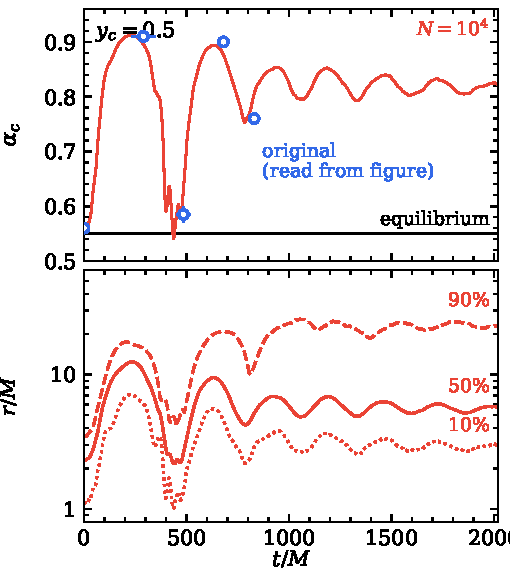
\includegraphics[width=\columnwidth]{figures/fig_migration.pdf}
\caption{The unperturbed cluster $y_c = 0.5$ expands, recontracts deeply, and oscillates with decreasing swing about a more extended state. Top: central lapse $\alpha_c$, equilibrium (black), and extrema from Ref.~\cite{Wu:2026nrpic} (circles; bars: read ranges). Bottom: radii enclosing the labeled rest-mass fractions.}
\label{fig:migration}
\end{figure}

Near the binding-energy maximum, Ref.~\cite{Wu:2026nrpic} applies a ten-percent initial density perturbation to $y_c = 0.756$ at $N = 10^6$. It reports reconfiguration into a persistent core--halo structure with all macroparticles retained, damped early lapse oscillations, and a slow fall of $\alpha_c$. Its text states the amplitude of the perturbation and leaves its sign and the initial-metric construction open. Over the shorter runs here, the comparison is limited to $\alpha_c$ and the enclosed rest-mass radii shown in Fig.~\ref{fig:nearcritical}. Here homologous radial scaling changes the density by ten percent of either sign while $\psi$ solves $\Ham = 0$ for the perturbed matter (Appendix~\ref{app:sampling}). Under ten-percent compression, the cluster contracts and collapses to a black hole with every macroparticle removed by lapse excision (Fig.~\ref{fig:nearcritical}; Tables~\ref{tab:setups} and \ref{tab:outcomes_migration}). The final apparent-horizon mass equals the ADM mass of the compressed initial data. A control run with the compressed particles on the unperturbed equilibrium metric contracts in the same way. Under ten-percent expansion, the cluster oscillates and keeps every macroparticle (Fig.~\ref{fig:nearcritical}). Its oscillation runs about a higher central lapse and with a slower rhythm than the published $\alpha_c$ curve of Ref.~\cite{Wu:2026nrpic}. The unperturbed model $y_c = 0.756$ oscillates about its equilibrium at the core period with a swing that grows and then stops growing (Fig.~\ref{fig:nearcritical}). Its mean lapse falls slowly below the equilibrium value over the run, as in the published $\alpha_c$ curve. That $\alpha_c$ evolution matches the core oscillation of the stable model in Fig.~\ref{fig:oscillation} and, apart from a time shift, resembles the published $\alpha_c$ curve in Ref.~\cite{Wu:2026nrpic} most closely (Table~\ref{tab:outcomes_migration}). As an interpretation, the oscillation in the published figure may be this intrinsic core oscillation, while which perturbation Ref.~\cite{Wu:2026nrpic} applied cannot be decided from its text.

\begin{figure}[t]
\centering
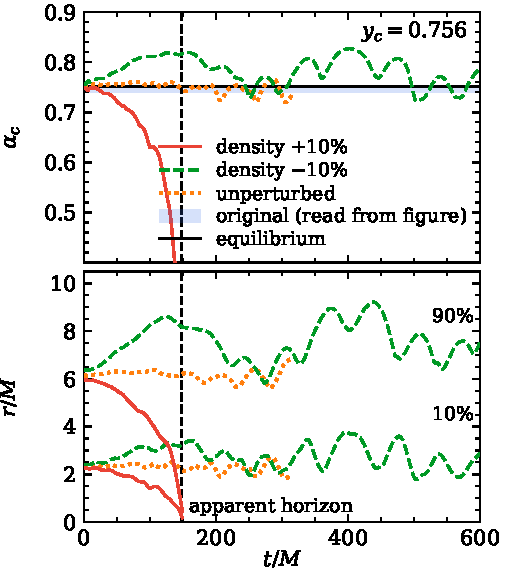
\includegraphics[width=\columnwidth]{figures/fig_nearcritical.pdf}
\caption{The near-critical cluster $y_c = 0.756$ collapses to a black hole when compressed, oscillates when expanded, and shows the core oscillation when unperturbed. Top: central lapse $\alpha_c$, first apparent horizon (dashed), and extrema from Ref.~\cite{Wu:2026nrpic} (circles). Bottom: radii enclosing the labeled rest-mass fractions.}
\label{fig:nearcritical}
\end{figure}
}{}
\IfFileExists{sections/assembly.tex}{\section{How the code was assembled}\label{sec:assembly}

The published text of the numerical-relativity particle-in-cell (NRPIC) method \cite{Wu:2026nrpic} provided the sole specification for the coupled Einstein-Vlasov solver built here without access to the original authors' code. This independent reconstruction tests whether the written equations and algorithmic rules fix the coupled method completely. The implementation assembles the coupled solver inside the host code AthenaK \cite{2026ApJS..283...27S,Zhu:2024utz} from existing capabilities across neighboring fields. AthenaK supplies the block-structured octree mesh with adaptive refinement, ghost-zone exchange, prolongation, and restriction. It also provides the Z4c spacetime solver in moving-puncture gauge, the particle container and drift update, the magnetohydrodynamics matter-source interface, and the pseudospectral apparent-horizon finder \cite{2026ApJS..283...27S,Zhu:2024utz}. Portable parallel execution of mesh stencils and particle loops comes from the Kokkos performance-portability library \cite{2022ITPDS..33..805T}.

Plasma particle-in-cell methods contribute implicit midpoint geodesic integration \cite{Bacchini:2020cze}, the velocity-space Boris rotation \cite{boris1970relativistic,1991ppcs.book.....B}, cloud-in-cell deposition with binomial filtering and compensation \cite{1988csup.book.....H,1991ppcs.book.....B}, and conservative single-level deposition across refinement boundaries \cite{Myers:2021gfn}. Numerical relativity and mesh methods supply the tetrad form of geodesic motion \cite{Olivares:2021cfa,Boyeneni:2025tsx}, lapse excision inside black holes \cite{Rosswog:2023nnl}, parabolic relaxation of the Hamiltonian constraint \cite{Duez:2002bn,Etienne:2024ncu}, and the L\"ohner refinement indicator \cite{1987CMAME..61..323L}. Exact analytical solutions for Kerr geodesics, Oppenheimer--Snyder dust collapse \cite{Oppenheimer:1939ue}, monoenergetic cluster equilibria \cite{1985ApJ...298...34S}, and homogeneous spheroid potentials complete the external inputs. This work combines those inputs into the two geodesic pushers in the symmetric and Cholesky tetrad gauges, cubic Hermite metric reconstruction, and single-level deposition with an optional level cap and compensated filtering. Additional components built here provide particle-coupled adaptive mesh refinement, lapse excision with interpolant-derivative apparent-horizon diagnostics, constraint-control terms, initial-data and validation suites, and the staggered coupled cycle.

Figure~\ref{fig:hypergraph} shows which capabilities each component combines. Horizontal rows list the existing capabilities grouped along the left margin by their origin. Vertical red columns represent the components built in this work as hyperedges of a hypergraph. Blue dots along each column mark the inherited capabilities joined by that hyperedge. Red rows at the bottom denote the geodesic-pusher and deposition components built here. Red dots on those bottom rows mark their reuse inside the adaptive-mesh and coupled-cycle hyperedges.

\begin{figure*}[t]
\centering
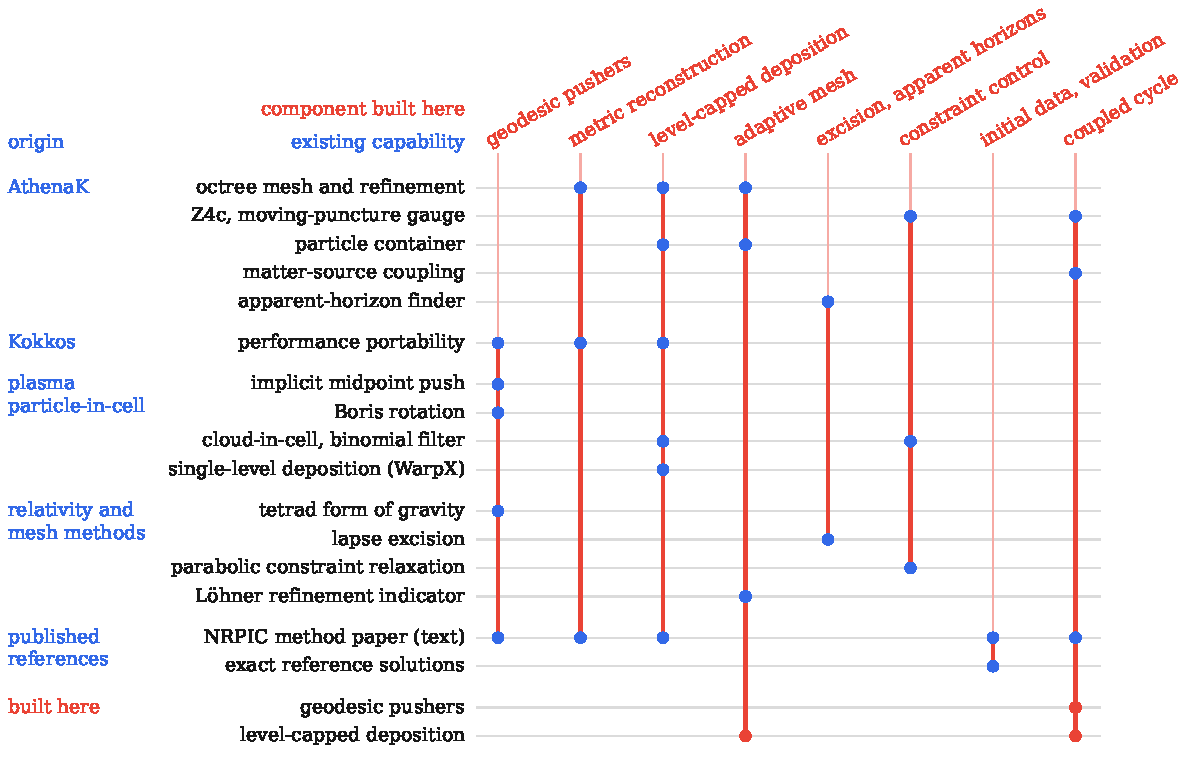
\includegraphics[width=\textwidth]{figures/fig_hypergraph.pdf}
\caption{The hypergraph shows how the code was assembled. Each row is a capability taken from an existing code or published method, grouped by origin. Each red column is a component built here, a hyperedge joining the capabilities it combines (dots). The red rows at the bottom are built components reused inside the coupled cycle and the adaptive mesh.}
\label{fig:hypergraph}
\end{figure*}

Large-language-model agents carried out the reconstruction under human direction across dedicated solver-development, verification, and manuscript roles. One model in the solver-development role wrote the derivations and solver source and directed the tests. Other models in the verification role built, ran, and analyzed the simulations, wrote independent reference solutions without access to the solver source, and audited the derivations, figures, and tables. A third model in the manuscript role wrote the text from the method specifications, figures, and test outcomes.

Candidate explanations for unexpected simulation results were tested against predictions recorded in advance. Each control run designed to test a stated explanation was preceded by a written prediction of the expected outcome. Seven initial explanations were refuted by these control runs. First, an apparent-horizon mass below $M$ after spherical collapse was attributed to early stopping of the pseudospectral flow finder. Calibration runs on an evolved vacuum black hole of known mass $M$ tested that explanation with a tighter stopping rule, which left the deficit unchanged. On the two finer meshes where the black hole is resolved, independent evaluations of the slice Misner--Sharp mass $M_{\rm MS}$ confirmed that the slice carried the mass $M$ (Fig.~\ref{fig:horizoncheck}; Table~\ref{tab:outcomes}). Direct inspection of the host code's finder showed that it interpolates a cell-centered metric-derivative array whose ghost zones retain their allocated zeros across mesh-block faces. Differentiation of the ghost-filled metric interpolant at those two cell sizes brought $M_{\rm AH}$ into agreement with $M_{\rm MS}$ on saved slices and in a live run. In Sec.~\ref{sec:dust}, three further initial explanations failed predictive controls: collapse dynamics for post-excision mass drift, harmlessness of one-level cloud coarsening, and the lattice beat alone for coarser-cloud disturbances. In Sec.~\ref{sec:clusters}, three more failed: sampling noise for the plain-filter bounce, sampling noise for the core oscillation, and second-order cell-size error for that oscillation. Independent audits of initial-data code and appendix tables against saved outputs caught two derivation slips and exposed unsupported log entries that were then corrected. In particular, redeposition from stored particles showed that a central-density excess under coarser clouds, first logged as matching the cycloid, came from the particle lattice beating against virtual cloud cells. Every effect without an isolating run has its cause stated in Sec.~\ref{sec:selfgravity} as not determined.

All materials needed to inspect and extend the simulations are public alongside the solver source code. The public release includes the simulation inputs, the analysis scripts, and the chronological record of every prediction and outcome. Readers can rerun the validation benchmarks, modify individual stages of the particle-mesh cycle, or audit each diagnostic test from those materials. The data-and-code-availability statement before the appendices gives the archive location.
}{}
\IfFileExists{sections/conclusions.tex}{\input{sections/conclusions}}{}

\IfFileExists{sections/acknowledgments.tex}{\section*{Data and code availability}

The solver source (a particle module inside the public code AthenaK \cite{2026ApJS..283...27S,Zhu:2024utz}), the inputs of every run, and the initial-data generators are public at \url{https://github.com/FoAKTEE/nrpic}.
The same repository provides the analysis and figure scripts alongside the data behind every figure.
It also holds the ledger of every number in the tables and the chronological record of predictions and outcomes.

\begin{acknowledgments}
This work rebuilds the method of Ref.~\cite{Wu:2026nrpic} from its published text, and we thank its authors for the level of detail of that text.
We acknowledge the developers of AthenaK \cite{2026ApJS..283...27S,Zhu:2024utz} and Kokkos \cite{2022ITPDS..33..805T} for the public host code and performance-portability library used here.
Large-language-model agents under human direction wrote the solver source, ran and analyzed the simulations, made the figures, and wrote the text.
One language-model family served each of the dedicated solver-development, verification, and manuscript roles described in Sec.~\ref{sec:assembly}.
The human authors directed the work and decided what was tested.
They take responsibility for the content of this paper.

% [Funding and computing-resource acknowledgments to be supplied by the authors.]
[Funding and computing-resource acknowledgments to be supplied by the authors.]
\end{acknowledgments}
}{}

\appendix
\IfFileExists{sections/appendix_parameters.tex}{\section{Scenario parameters and measured values}\label{app:parameters}

Table~\ref{tab:setups} lists the setup of every family of runs. Tables~\ref{tab:outcomes} and \ref{tab:outcomes_clusters} list the measured values to which the text refers, with the values of Ref.~\cite{Wu:2026nrpic} where it gives them.

\begin{table*}
\caption{Setups, one row per family of runs: model, macroparticle number $N$ and sampling, domain half-width $L$, mesh and cell spacing $\Delta x$ in the matter at the start and the finest reached (vacuum runs: at the puncture), first time step $\Delta t$, filter passes $n_{\rm f}$ (+c: compensation pass), deposition, excision threshold $\aexc$, constraint damping $\kappa_1$, final time. Meshes other than uniform have $64^3$ root cells in MeshBlocks of $16^3$ cells. Parentheses: single runs of a family.}
\label{tab:setups}
\footnotesize
\setlength{\tabcolsep}{2pt}
\begin{ruledtabular}
\begin{tabular}{p{0.22\textwidth}p{0.1\textwidth}p{0.05\textwidth}p{0.135\textwidth}p{0.07\textwidth}p{0.06\textwidth}p{0.085\textwidth}p{0.035\textwidth}p{0.065\textwidth}p{0.065\textwidth}}
\raggedright Scenario and model & \raggedright $N$, sampling & \raggedright $L/M$ & \raggedright Mesh, $\Delta x/M$ & \raggedright $\Delta t/M$ & \raggedright $n_{\rm f}$ & \raggedright Deposition & \raggedright $\aexc$ & \raggedright $\kappa_1$ & \raggedright $t_{\rm end}/M$ \tabularnewline
\colrule
\raggedright Kerr geodesics: $a=0.9M$, $a\to0$; bound, $e=0.99$, plunging & \raggedright 1 & \raggedright 10--12 & \raggedright uniform, 1/8--1/2; lattice 0.025 & \raggedright 0.00125--0.08 & \raggedright -- & \raggedright -- & \raggedright -- & \raggedright -- & \raggedright 77.5--4550 \tabularnewline
\raggedright Test-particle clusters: $a=0.9M$, $a\to0$; cloud at $r_0=10M$ & \raggedright $10^2$--$10^4$, Gaussian & \raggedright 64 & \raggedright static, 1/4$\to$1/16 & \raggedright 0.05 & \raggedright 2 & \raggedright finest level & \raggedright 0.62 & \raggedright -- & \raggedright 500--1000 \tabularnewline
\raggedright Vacuum black hole: puncture of mass $M$; 6 tracers & \raggedright 6, tracers & \raggedright 128 & \raggedright static, 1/8 (1/4, 1/16) & \raggedright 1/32 (1/16, 1/64) & \raggedright -- & \raggedright none & \raggedright 0.05 & \raggedright 0.02 & \raggedright 12--250 \tabularnewline
\raggedright Head-on collision: punctures $M/2$ at $x=\pm5M$; 6 tracers & \raggedright 6, tracers & \raggedright 128 & \raggedright adaptive, 1/16 & \raggedright 1/64 & \raggedright -- & \raggedright none & \raggedright 0.05 & \raggedright 0.02 & \raggedright 160 \tabularnewline
\raggedright Dust collapse: $R_0=5M$, $h=0.30M$; masses corrected, published & \raggedright 9328, lattice & \raggedright 155 & \raggedright adaptive, 0.30$\to$0.038 & \raggedright 0.076 & \raggedright 1 & \raggedright finest level & \raggedright 0.1 & \raggedright 0.02 & \raggedright 60 \tabularnewline
\raggedright Dust collapse, level cap: as above, corrected masses & \raggedright 9328, lattice & \raggedright 155 & \raggedright adaptive, 0.30$\to$0.038 & \raggedright 0.076 & \raggedright 1 & \raggedright level-capped ($\le1$, $\le2$, any) & \raggedright 0.1 & \raggedright 0.02 & \raggedright 60 \tabularnewline
\raggedright Stable cluster, filter: $y_c=0.819$, unperturbed; samples 1--3 & \raggedright $10^4$, stratified & \raggedright 1024 & \raggedright static, 1/2 & \raggedright 1/8 & \raggedright 0, 2, 2+c, 4, 4+c & \raggedright finest level & \raggedright 0.1 & \raggedright 0.02 & \raggedright 300 \tabularnewline
\raggedright Stable cluster, oscillation: $y_c=0.819$, unperturbed; sample 1 & \raggedright $10^4$, stratified & \raggedright 1024 & \raggedright static, 1/2 (1/4--1/2) & \raggedright 1/8 (1/16) & \raggedright 4+c\footnotemark[2] & \raggedright finest level & \raggedright 0.1 & \raggedright 0.02 (0.1, 0)\footnotemark[1] & \raggedright 300--1200 \tabularnewline
\raggedright Particle number: $y_c=0.819$; kick 0.01 or none & \raggedright $10^2$--$10^4$, Monte Carlo, stratified & \raggedright 1024 & \raggedright static, 1/2 & \raggedright 1/8 & \raggedright 4+c & \raggedright finest level & \raggedright 0.1 & \raggedright 0.02 & \raggedright 300--500 \tabularnewline
\raggedright Sequence, stable: $y_c=0.900, 0.819$; kick 0.01 & \raggedright $10^4$, stratified & \raggedright 1024 & \raggedright static, 1/2 & \raggedright 1/8 & \raggedright 4+c & \raggedright finest level & \raggedright 0.1 & \raggedright 0.02 & \raggedright 300 \tabularnewline
\raggedright Sequence, unstable: $y_c=0.605, 0.500, 0.283$; kick 0.01 & \raggedright $10^4$, stratified & \raggedright 512 & \raggedright adaptive, 1/4$\to$1/16 & \raggedright 1/16 & \raggedright 4+c & \raggedright finest level & \raggedright 0.1 & \raggedright 0.02 & \raggedright 120--300 \tabularnewline
\raggedright Unperturbed unstable: $y_c=0.500$, unperturbed; samples 1--3 & \raggedright $10^4$, stratified & \raggedright 512 & \raggedright static, 1/4 & \raggedright 1/16 & \raggedright 4, 4+c & \raggedright finest level & \raggedright 0.1 & \raggedright 0.02 & \raggedright 200--2429\footnotemark[3] \tabularnewline
\raggedright Near-critical: $y_c=0.756$; density $\times(1\pm0.1)$ & \raggedright $10^4$, stratified & \raggedright 512 (1024) & \raggedright adaptive, 1/4$\to$1/16 (adaptive, 1/4; static, 1/4) & \raggedright 1/16 & \raggedright 4+c & \raggedright finest level & \raggedright 0.1 & \raggedright 0.02 & \raggedright 160--818 \tabularnewline
\end{tabular}
\end{ruledtabular}
\footnotetext[1]{One run adds parabolic relaxation of $\Ham$ with $c_H=0.05\,M$.}
\footnotetext[2]{One run uses $c=n_{\rm f}/4+1/12$, which also cancels the cloud width.}
\footnotetext[3]{Run in progress; values up to its last record.}
\end{table*}

\begin{table*}
\caption{Measured quantities to which the text refers for test particles, the apparent-horizon check and dust collapse, with the values of Ref.~\cite{Wu:2026nrpic} where it gives them (from its text, or read from its figures). Masses in units of the total mass $M$, times in units of $M$; listed values follow the order named in the first column.}
\label{tab:outcomes}
\footnotesize
\setlength{\tabcolsep}{3pt}
\begin{ruledtabular}
\begin{tabular}{p{0.49\textwidth}p{0.26\textwidth}p{0.205\textwidth}}
Quantity & This work & Ref.~\cite{Wu:2026nrpic} \tabularnewline
\colrule
\multicolumn{3}{l}{\textit{Fixed black hole}} \tabularnewline
\raggedright Passage $e=0.99$, largest relative errors of $\Egeo$, $L_z$, $Q$ ($\Delta t=0.01M$, to $230M$): & \raggedright  & \raggedright  \tabularnewline
\raggedright \quad implicit midpoint, analytic metric & \raggedright $2.78\times10^{-8}$, $0$, $1.25\times10^{-7}$ & \raggedright $2.8\times10^{-8}$, round-off, $1.3\times10^{-7}$ \tabularnewline
\raggedright \quad spacetime Boris, symmetric gauge, analytic & \raggedright $9.05\times10^{-8}$, $1.14\times10^{-8}$, $7.83\times10^{-7}$ & \raggedright $9.0\times10^{-8}$, $1.1\times10^{-8}$, $7.8\times10^{-7}$ \tabularnewline
\raggedright \quad implicit midpoint, Hermite lattice & \raggedright $2.16\times10^{-6}$, $5.30\times10^{-6}$, $5.06\times10^{-5}$ & \raggedright $2.2\times10^{-6}$, $5.3\times10^{-6}$, $5.1\times10^{-5}$ \tabularnewline
\raggedright \quad spacetime Boris, Cholesky gauge, Hermite lattice & \raggedright $2.05\times10^{-6}$, $3.79\times10^{-6}$, $5.29\times10^{-5}$ & \raggedright $2.0\times10^{-6}$, $3.8\times10^{-6}$, $5.3\times10^{-5}$ \tabularnewline
\raggedright Passage, order of convergence in $\Delta t$ (three pushers, analytic metric) & \raggedright 1.995--2.001 & \raggedright second order \tabularnewline
\raggedright Inclined Kerr orbit on the mesh, order in $h$ of position and $\Egeo$ errors & \raggedright 2.89, 3.29 & \raggedright -- \tabularnewline
\raggedright Plunging clusters ($N=10^4$): removed by excision, against exact geodesics; $a\to0$ and $a=0.9M$ & \raggedright 3726 vs 3727; 3345 vs 3339 & \raggedright -- \tabularnewline
\raggedright Bound clusters, exponent of the filtered-$E$ differences against $N$; $a\to0$ and $a=0.9M$ & \raggedright $-0.48$, $-0.48$ & \raggedright -- \tabularnewline
\colrule
\multicolumn{3}{l}{\textit{Evolving black holes}} \tabularnewline
\raggedright Puncture: largest relative change of $L_z$ of the four circular tracers & \raggedright $1.1\times10^{-4}$--$3.9\times10^{-4}$ & \raggedright -- \tabularnewline
\raggedright Puncture: radial infall and plunge removed at $\aexc$, $t/M$ & \raggedright 54, 126 & \raggedright -- \tabularnewline
\raggedright Puncture ($\Delta x=M/8$), slice Misner--Sharp horizon mass at $t=50M$ & \raggedright 1.0016 & \raggedright -- \tabularnewline
\raggedright Head-on: first common apparent horizon $t/M$; its mass at the end & \raggedright 49.25; 1.0026 & \raggedright -- \tabularnewline
\raggedright Head-on: largest relative change of $L_x$ (five orbiting tracers); $|L_x|$ of the tracer from rest & \raggedright $9.8\times10^{-4}$; $4\times10^{-14}$ & \raggedright -- \tabularnewline
\colrule
\multicolumn{3}{l}{\textit{Apparent-horizon check}} \tabularnewline
\raggedright Finder as distributed, $t=50M$, at $\Delta x=M/4$, $M/8$, $M/16$ & \raggedright 0.9353, 0.9771, 0.9406 & \raggedright -- \tabularnewline
\raggedright Slice Misner--Sharp horizon mass, same slices & \raggedright 0.9656, 1.0016, 1.0000 & \raggedright -- \tabularnewline
\raggedright Finder as distributed ($M/8$), stopping tolerance $10^{-5}$ and $10^{-8}$, $t\simeq50M$ & \raggedright 0.9771, 0.9771 & \raggedright -- \tabularnewline
\raggedright Corrected finder in a live run ($M/8$), last search; slice mass at $t=12M$ & \raggedright 1.0003; 1.0006 & \raggedright -- \tabularnewline
\colrule
\multicolumn{3}{l}{\textit{Dust collapse}} \tabularnewline
\raggedright Central proper time $\tau_c/M$ at which $\alpha_c$ exceeds the lapse bound by $10^{-2}$ & \raggedright 3.53 & \raggedright $\simeq3.5$ \tabularnewline
\raggedright Rest mass $\sum_p m_p/M$: published lattice rule; surface-corrected (continuum $M_0$) & \raggedright 1.1687; 1.1551 & \raggedright $\simeq1.155$ ($N\simeq10^6$) \tabularnewline
\raggedright First apparent horizon $t/M$ (finest-level clouds, corrected masses) & \raggedright 16.39 & \raggedright -- \tabularnewline
\raggedright $M_{\rm AH}/M$ at formation; at $t=60M$ (finest-level clouds, corrected masses) & \raggedright 1.0004; 0.9987 & \raggedright $|M_{\rm AH}/M-1|\lesssim10^{-3}$ at $60M$ \tabularnewline
\raggedright $M_{\rm AH}/M$ at formation; at $t=60M$ (published lattice masses) & \raggedright 1.0114; 1.0099 & \raggedright -- \tabularnewline
\raggedright $M_{\rm AH}/M$ when the last macroparticle is removed $\to$ at $t=60M$: finest level; level cap with any, $\le2$, $\le1$ levels of coarsening & \raggedright 1.0004$\to$0.9987; 1.0006$\to$1.0065; 1.0006$\to$1.0064; 1.0012$\to$0.9904 & \raggedright -- \tabularnewline
\raggedright Largest $\|\Ham\|$, same four runs & \raggedright 1.9, 4.7, 4.5, 2.8 & \raggedright -- \tabularnewline
\raggedright Largest $\|\Ham\|$ within $1M$ after the refinement to $\Delta x=h/4$, same four runs & \raggedright 1.59, 0.48, 0.48, 1.14 & \raggedright -- \tabularnewline
\raggedright $E_c$ over the cycloid in the $3M$ after the refinement to $h/4$: finest level; level cap with any, $\le1$ levels & \raggedright 0.27--0.52; 1.11--1.14; 1.28--1.49 & \raggedright -- \tabularnewline
\end{tabular}
\end{ruledtabular}
\end{table*}

\begin{table*}
\caption{As Table~\ref{tab:outcomes}, for the relativistic clusters. Central lapse $\alpha_c$ in the eight central cells; $\alpha_c(0)$ is its value at $t=0$.}
\label{tab:outcomes_clusters}
\footnotesize
\setlength{\tabcolsep}{3pt}
\begin{ruledtabular}
\begin{tabular}{p{0.49\textwidth}p{0.26\textwidth}p{0.205\textwidth}}
Quantity & This work & Ref.~\cite{Wu:2026nrpic} \tabularnewline
\colrule
\multicolumn{3}{l}{\textit{Stable cluster $y_c=0.819$: filter}} \tabularnewline
\raggedright Rise of $\alpha_c$ above $\alpha_c(0)$ within $130M$, sample 1, $n_{\rm f}=0$, 2, 4, 2+c, 4+c & \raggedright 0.0044, 0.0176, 0.0273, 0.0061, 0.0065 & \raggedright $\approx0.01$ (read from figure) \tabularnewline
\raggedright Same rise, samples 1--3, four plain passes; with compensation & \raggedright 0.0273, 0.0289, 0.0275; 0.0065, 0.0084, 0.0061 & \raggedright -- \tabularnewline
\raggedright Filtered over deposited proper-volume integral of $E$, minus one: four plain passes; with compensation & \raggedright $-3.0\times10^{-3}$; $-1.0\times10^{-4}$ & \raggedright -- \tabularnewline
\raggedright $\|\Ham\|$ at $t=300M$: no filter; four plain passes; with compensation & \raggedright 0.141; 0.011; 0.031 & \raggedright -- \tabularnewline
\colrule
\multicolumn{3}{l}{\textit{Stable cluster $y_c=0.819$: core oscillation}} \tabularnewline
\raggedright Period of $\alpha_c$ ($100$--$1200M$); radial period in the core, $\pi[3/(4\pi E_c)]^{1/2}$ & \raggedright 75; 66 & \raggedright -- \tabularnewline
\raggedright Half the swing of $\alpha_c$ in windows of $100M$: growth phase ($100$--$500M$); after $500M$ & \raggedright 0.005$\to$0.018; 0.015--0.022 & \raggedright -- \tabularnewline
\raggedright Largest $|\Delta\alpha_c|$ from sample 1 over $300M$: $\Delta t/2$, $\kappa_1=0.1$, $\kappa_1=0$, $c_H$ & \raggedright $6.5\times10^{-4}$, $3.1\times10^{-4}$, $7.9\times10^{-5}$, $2.1\times10^{-5}$ & \raggedright -- \tabularnewline
\raggedright Same, compensation that also cancels the cloud width & \raggedright $3.6\times10^{-3}$ & \raggedright -- \tabularnewline
\raggedright Near-critical $y_c=0.756$ in Ref.~\cite{Wu:2026nrpic}: period of $\alpha_c$; here the core radial period of that model & \raggedright 45 & \raggedright $\approx50$ (read from figure) \tabularnewline
\colrule
\multicolumn{3}{l}{\textit{Stable cluster $y_c=0.819$: particle number}} \tabularnewline
\raggedright Monte Carlo, $N=10^3$ against $10^4$: largest difference of $\alpha_c-\alpha_c(0)$ to $190M$; lowest $\alpha_c-\alpha_c(0)$ after $190M$ ($10^4$, $10^3$); mean over $400$--$500M$ ($10^4$, $10^3$) & \raggedright 0.005; $-0.023$, $-0.035$; $-0.003$, $-0.017$ & \raggedright -- \tabularnewline
\raggedright Monte Carlo $N=10^2$: $\alpha_c$ at $t=0$, $200M$, $500M$; mean Lorentz factor at start and end; largest $|\sum_p m_p u_{i,p}|/M_0$ & \raggedright 0.81, 0.68, 0.58; 1.047, 1.138; 0.039 & \raggedright -- \tabularnewline
\colrule
\multicolumn{3}{l}{\textit{Cluster sequence with inward kick}} \tabularnewline
\raggedright $\alpha_c$ range over $300M$, $y_c=0.900$; $0.819$; particles kept & \raggedright 0.886--0.892; 0.787--0.819; all & \raggedright $\approx0.89$; $0.81$--$0.82$ (read from figure) \tabularnewline
\raggedright First apparent horizon $t/M$: $y_c=0.605$; $0.500$ & \raggedright 191.0; 104.3 & \raggedright 109; 73 \tabularnewline
\raggedright $M_{\rm AH}/M$ at the end; macroparticles left of $10^4$ & \raggedright 1.0000; 1.0001; 6, 3 & \raggedright $\simeq1$ (stated) \tabularnewline
\raggedright $\alpha_c$ at the end, after the horizon forms: $y_c=0.605$; $0.500$ & \raggedright 0.051; 0.016 & \raggedright $\approx0.20$ (read from figure) \tabularnewline
\raggedright $y_c=0.283$: $\alpha_c$ at the end ($t/M$); particles kept & \raggedright 0.976 (270); all & \raggedright $\approx0.98$ (300; read from figure) \tabularnewline
\colrule
\multicolumn{3}{l}{\textit{Unperturbed $y_c=0.5$}} \tabularnewline
\raggedright Time $t/M$ at which $\alpha_c$ first reaches 0.8: plain filter; compensated, samples 1--3 & \raggedright 59; 88, 86, 91 & \raggedright $\approx120$ (read from figure) \tabularnewline
\raggedright Migration, $\alpha_c$ at the start and at its first extrema ($t/M$) & \raggedright 0.55; 0.91 (228); 0.54 (437); 0.89 (632); 0.75 (783) & \raggedright 0.56; 0.91 (230--320); 0.55--0.56 (450--490); 0.90 (670); 0.76 (830) (read from figure) \tabularnewline
\raggedright Migration (run in progress, records to $t/M$ given): macroparticles removed by excision; leaving the domain (at $t/M$) & \raggedright 0; 3 (1816, 1999, 2405); to 2429 & \raggedright -- \tabularnewline
\colrule
\multicolumn{3}{l}{\textit{Near-critical $y_c=0.756$}} \tabularnewline
\raggedright Compressed by ten percent: $\alpha_c(0)$; first apparent horizon $t/M$ & \raggedright 0.749; 147.2 & \raggedright $\simeq0.75$; none \tabularnewline
\raggedright Compressed: $M_{\rm AH}/M$ at the end; $M$ of the initial data; macroparticles left & \raggedright 0.9970; 0.9969; 0 & \raggedright all kept \tabularnewline
\raggedright Compressed: largest $|\Delta\alpha_c|$ to $120M$ between the consistent and the unperturbed initial metric & \raggedright 0.009 & \raggedright -- \tabularnewline
\end{tabular}
\end{ruledtabular}
\end{table*}

}{}
\IfFileExists{sections/appendix_sampling.tex}{\section{Initial data and sampling}\label{app:sampling}

Coupled Einstein-Vlasov evolutions require constraint-satisfying initial slices alongside discrete particle ensembles that sample the continuum phase-space distribution. Each self-gravitating run starts on a conformally flat, time-symmetric slice where superposed flat-space Poisson potentials $u_c$ for conformal sources $\tilde{\rho}_c$ solve $\Ham=0$ via Eq.~(\ref{eq:initial_superposition}). Around each component center $\bm{x}_c$ at isotropic distance $\rbar_c=|\bm{x}-\bm{x}_c|$, four component families enter Eq.~(\ref{eq:initial_superposition}). Tabulated spherical profiles interpolate $u_c(\rbar_c)=\psi_c(\rbar_c)-1$ on a uniform grid with four-point Lagrange polynomials and follow Eq.~(\ref{eq:puncture_potential}) outside with the component ADM mass. Vacuum black hole punctures evaluate Eq.~(\ref{eq:puncture_potential}) directly, while spherical Gaussian components of conformal mass $m_c$ and width $\sigma_c$ obey
\begin{align}\label{eq:app_gaussian}
\tilde{\rho}_c(\rbar_c)&=\frac{m_c}{(2\pi\sigma_c^2)^{3/2}}\exp\!\left(-\frac{\rbar_c^2}{2\sigma_c^2}\right),\nonumber\\
u_c(\rbar_c)&=\frac{m_c}{2\rbar_c}\,\mathrm{erf}\!\left(\frac{\rbar_c}{\sqrt{2}\,\sigma_c}\right).
\end{align}
A homogeneous prolate spheroid of ADM mass $M$, polar semi-axis $b$ along $z$, eccentricity $e$, equatorial semi-axis $a_{\mathrm{eq}}=b\sqrt{1-e^2}$, and focal half-distance $d_{\mathrm{f}}=eb$ has closed-form fields \cite{Shapiro:1991zza,Yoo:2016kzu}
\begin{align}\label{eq:app_spheroid}
\tilde{\rho}_c(\bm{x})&=\frac{3M}{4\pi a_{\mathrm{eq}}^2b},\qquad\frac{x^2+y^2}{a_{\mathrm{eq}}^2}+\frac{z^2}{b^2}\le1,\nonumber\\
u_c(\bm{x})&=\frac{3M}{8}\Bigl[I_0(\lambda)-(x^2+y^2)J_{\mathrm{eq}}(\lambda)-z^2J_z(\lambda)\Bigr],\nonumber\\
I_0(\lambda)&=\frac{2}{d_{\mathrm{f}}}\,\mathrm{arctanh}\!\left(\frac{d_{\mathrm{f}}}{b_\lambda}\right),\nonumber\\
J_{\mathrm{eq}}(\lambda)&=\frac{b_\lambda}{d_{\mathrm{f}}^2(a_{\mathrm{eq}}^2+\lambda)}-\frac{I_0(\lambda)}{2d_{\mathrm{f}}^2},\nonumber\\
J_z(\lambda)&=\frac{I_0(\lambda)}{d_{\mathrm{f}}^2}-\frac{2}{d_{\mathrm{f}}^2b_\lambda},\nonumber\\
1&=\frac{x^2+y^2}{a_{\mathrm{eq}}^2+\lambda}+\frac{z^2}{b^2+\lambda}\qquad(\lambda>0).
\end{align}
The auxiliary length $b_\lambda=\sqrt{b^2+\lambda}$ sets $\lambda=0$ inside the spheroid, while outside the boundary $\tilde{\rho}_c$ vanishes and $\lambda>0$ solves the last relation. Every initial slice sets vanishing shift $\beta^i=0$, with initial lapse $\alpha=1$ for cold collapse and $\alpha=\psi^{-2}$ for vacuum punctures. Isolated clusters use their static equilibrium lapse joined outside to $(1-u_c)(1+u_c)^{-1}$, whereas the composite cluster uses $\alpha=2\psi^{-1}-1$. Since $\sqrt{\gamma}=\psi^6$, $N$ equal-mass macroparticles sampling proper rest-mass density $\rho_0$ and continuum rest mass $M_0$ have coordinate number density
\begin{align}\label{eq:app_coord_density}
\mathcal{N}(\bm{x})&=\frac{N}{M_0}\,\rho_0(\bm{x})\psi(\bm{x})^6,\nonumber\\
m_p&=\frac{M_0}{N},\qquad M_0=\int\rho_0(\bm{x})\psi(\bm{x})^6\,\dd^3x.
\end{align}
For the cold prolate spheroid ($u_{i,p}=0$, $\rho_0\psi^6=\tilde{\rho}_c\psi$), one quarter of the $N$ particles are drawn inside the boundary by rejection against $\psi(\bm{x})\psi(\bm{0})^{-1}$ and completed by $(x,y,-z)$ and $(-x,-y,\pm z)$. Gaussian components draw positions around $\bm{x}_c$ by randomized stratification in radius and angles. In multi-component superpositions, each component multiplies its isolated particle masses by $\psi\psi_c^{-1}$ ($\psi_c=1$ and rest mass $m_cW_c^{-1}$ at bulk Lorentz factor $W_c$) and lowers orthonormal momenta with $\psi^2$.

The homogeneous dust ball of mass $M$, areal radius $R_0$, and density $\rho_0$ (Sec.~\ref{sec:dust}) starts from rest ($u_{i,p}=0$) with isotropic radius $\rbar_0$ and interior conformal factor \cite{Staley:2011ss}
\begin{align}\label{eq:app_dust_psi}
\rbar_0&=\frac{R_0}{2}\!\left(1-\frac{M}{R_0}+\sqrt{1-\frac{2M}{R_0}}\right),\nonumber\\
\psi(\rbar)&=\sqrt{\frac{\bigl(1+\sqrt{1-2M/R_0}\bigr)\rbar_0R_0^2}{2\rbar_0^3+M\rbar^2}}\qquad(\rbar\le\rbar_0),
\end{align}
matched to Eq.~(\ref{eq:puncture_potential}) outside. The cube $[-\rbar_0,\rbar_0]^3$ is partitioned into $n_{\mathrm{lat}}^3$ cubic cells of spacing $h=2\rbar_0n_{\mathrm{lat}}^{-1}$ aligned with the initial matter-level mesh, with $n_{\mathrm{lat}}$ in the parameter table. Macroparticles occupy cell centers with $\rbar_p=|\bm{x}_p|\le\rbar_0$ for noise-free interior deposition, and the published rule \cite{Wu:2026nrpic} assigns proper cell masses
\begin{equation}\label{eq:app_dust_published}
m_p^{\mathrm{pub}}=\rho_0\psi(\rbar_p)^6h^3.
\end{equation}
The count of lattice sites inside a sphere differs from its volume in cells $h^3$ by a boundary fraction of order $n_{\mathrm{lat}}^{-1}$, so summed $m_p^{\mathrm{pub}}$ exceeds $M_0$ on small lattices. Our surface correction leaves interior masses unchanged for $\rbar_p\le\rbar_0-h$ and rescales the outermost layer $\rbar_0-h<\rbar_p\le\rbar_0$ of width $h$ by one common factor so all particle masses sum to $M_0$,
\begin{equation}\label{eq:app_dust_surface}
m_p=m_p^{\mathrm{pub}}\,\frac{M_0-\sum_{\rbar_{p'}\le\rbar_0-h}m_{p'}^{\mathrm{pub}}}{\sum_{\rbar_{p'}>\rbar_0-h}m_{p'}^{\mathrm{pub}}}.
\end{equation}

Monoenergetic equilibrium clusters \cite{1985ApJ...298...34S} populate a single conserved energy per unit rest mass $E_0=\alpha_{\mathrm{s}}$ in Eq.~(\ref{eq:cluster_sequence}) with isotropic momentum directions. In dimensionless areal radius $\tilde{r}$, squared lapse ratio $y(\tilde{r})$ with $y(0)=y_c$, and enclosed gravitational and rest-mass variables $\tilde{m}$ and $\tilde{m}_0$, the structure equations and isotropic-radius map take the form
\begin{align}\label{eq:app_structure}
\zeta&=\frac{1-y_c}{3},\qquad g_y=\frac{y^{-1}-1}{y_c^{-1}-1},\nonumber\\
\frac{\dd y}{\dd\tilde{r}}&=\frac{2\zeta y}{\tilde{r}^2}\,\frac{\tilde{m}+\zeta\tilde{r}^3(y/y_c)^{-1/2}g_y^{3/2}}{1-2\zeta\tilde{m}/\tilde{r}},\nonumber\\
\frac{\dd\tilde{m}}{\dd\tilde{r}}&=\tilde{r}^2\!\left(\frac{y}{y_c}\right)^{\!-3/2}g_y^{1/2},\nonumber\\
\frac{\dd\tilde{m}_0}{\dd\tilde{r}}&=\frac{\tilde{r}^2y_c^{1/2}(y/y_c)^{-1}g_y^{1/2}}{\sqrt{1-2\zeta\tilde{m}/\tilde{r}}},\nonumber\\
\frac{\dd\ln\rbar}{\dd\ln\tilde{r}}&=\frac{1}{\sqrt{1-2\zeta\tilde{m}/\tilde{r}}}.
\end{align}
Near the cluster surface where density vanishes, the variable $\sqrt{1-y}$ keeps every derivative analytic up to $y(\tilde{r}_{\mathrm{s}})=1$. Outward integration from $\tilde{r}=0$ ($\tilde{m}=\tilde{m}_0=0$) yields surface values $(\tilde{r}_{\mathrm{s}},\tilde{m}_{\mathrm{s}},\tilde{m}_{0,\mathrm{s}})$ and interior profiles matched at $\rbar_{\mathrm{s}}$ from Eq.~(\ref{eq:app_dust_psi}),
\begin{align}\label{eq:app_cluster_profiles}
R&=\frac{M\tilde{r}_{\mathrm{s}}}{\zeta\tilde{m}_{\mathrm{s}}},\qquad M_0=\frac{M\tilde{m}_{0,\mathrm{s}}}{\tilde{m}_{\mathrm{s}}},\nonumber\\
E_0&=\sqrt{1-\frac{2M}{R}},\qquad\alpha_{\mathrm{eq}}(\rbar)=E_0\sqrt{y},\nonumber\\
\psi_{\mathrm{eq}}(\rbar)&=\sqrt{\frac{R\tilde{r}}{\tilde{r}_{\mathrm{s}}\rbar}},
\end{align}
with enclosed masses $m_{\mathrm{g}}=M\tilde{m}\tilde{m}_{\mathrm{s}}^{-1}$, $m_0=M_0\tilde{m}_0\tilde{m}_{0,\mathrm{s}}^{-1}$, and $4\pi\rbar^2\rho_0\psi_{\mathrm{eq}}^6\,\dd\rbar=\dd m_0$. For $N$ equal-mass macroparticles ($p=1,\dots,N$) and five coordinates $d\in\{1,\dots,5\}$, randomized stratification draws
\begin{equation}\label{eq:app_stratified}
U_{pd}=\frac{\pi_d(p)+\xi_{pd}}{N},
\end{equation}
where independent random permutations $\pi_d$ map $\{1,\dots,N\}$ onto $\{0,\dots,N-1\}$ and $\xi_{pd}$ is uniform on $[0,1)$. The cumulative rest-mass fraction $F(\rbar)=m_0(\rbar)M_0^{-1}$ sets each radial coordinate through $\rbar_p=F^{-1}(U_{p1})$. Position angles $(\cos\theta_p,\phi_p)=(2U_{p2}-1,2\pi U_{p3})$ define the radial unit vector $\hat{\bm{r}}_p$ and $\bm{x}_p=\rbar_p\hat{\bm{r}}_p$, while momentum angles $(\cos\theta_{u,p},\phi_{u,p})=(2U_{p4}-1,2\pi U_{p5})$ define an isotropic unit vector $\hat{\bm{u}}_p$. At radius $\rbar_p$, the monoenergetic condition $E_0=\alpha_{\mathrm{eq}}(\rbar_p)W_p$ and Eq.~(\ref{eq:lorentz_factor}) fix the local orthonormal momentum magnitude $u_{\mathrm{eq}}(\rbar_p)$ and covariant momentum,
\begin{align}\label{eq:app_cluster_momentum}
u_{\mathrm{eq}}(\rbar)&=\sqrt{\frac{E_0^2}{\alpha_{\mathrm{eq}}(\rbar)^2}-1},\nonumber\\
u_{i,p}&=\psi_{\mathrm{eq}}(\rbar_p)^2u_{\mathrm{eq}}(\rbar_p)\hat{u}_{i,p}.
\end{align}
Plain Monte Carlo sampling, used as the alternative in the particle-number study, replaces $U_{pd}$ in Eq.~(\ref{eq:app_stratified}) with independent uniform draws on $[0,1)$. Because the mass-weighted mean momentum of a finite sample does not vanish and makes the cluster drift, that mean is subtracted from every particle,
\begin{equation}\label{eq:app_zero_momentum}
u_{i,p}\leftarrow u_{i,p}-\frac{\sum_{p'=1}^{N}m_{p'}u_{i,p'}}{\sum_{p'=1}^{N}m_{p'}}.
\end{equation}

Along the equilibrium sequence, an inward velocity kick of fractional amplitude $\delta_v$ scales the radial momentum component as in Ref.~\cite{Wu:2026nrpic}, shifting $\hat{u}_{i,p}$ in Eq.~(\ref{eq:app_cluster_momentum}) to $\hat{u}_{i,p}-\delta_v\hat{r}_{i,p}$ before Eq.~(\ref{eq:app_zero_momentum}). For the homologous density perturbation $\delta_\rho$ of the near-critical model, equilibrium radii $\rbar_{\mathrm{eq},p}$ scale by a common factor $\Lambda_{\mathrm{h}}$ to $\rbar_p=\Lambda_{\mathrm{h}}\rbar_{\mathrm{eq},p}$ with $\bm{x}_p=\rbar_p\hat{\bm{r}}_p$. Unlike a perturbation applied on the unperturbed metric $\psi_{\mathrm{eq}}$, here $\psi(\rbar)$ is recomputed from the perturbed matter by a radial fixed-point solve of the Hamiltonian constraint,
\begin{align}\label{eq:app_perturbed_hc}
\Lambda_{\mathrm{h}}&=(1+\delta_\rho)^{-1/3},\nonumber\\
\frac{1}{\rbar^2}\frac{\dd}{\dd\rbar}\!\left(\rbar^2\frac{\dd\psi}{\dd\rbar}\right)&=-\frac{2\pi}{\Lambda_{\mathrm{h}}^3\psi(\rbar)}\,\rho_0\!\left(\frac{\rbar}{\Lambda_{\mathrm{h}}}\right)\psi_{\mathrm{eq}}\!\left(\frac{\rbar}{\Lambda_{\mathrm{h}}}\right)^{\!6}\bigl\langle W(\rbar)\bigr\rangle.
\end{align}
Outside $\Lambda_{\mathrm{h}}\rbar_{\mathrm{s}}$, $\psi(\rbar)$ joins $1+M'(2\rbar)^{-1}$ for perturbed ADM mass $M'$, while the interior lapse rescales $\alpha_{\mathrm{eq}}(\rbar\Lambda_{\mathrm{h}}^{-1})$ continuously to the exterior isotropic Schwarzschild lapse. Particle momenta at $\rbar_p$ are set from $E_0$ via $u_{\mathrm{eq}}(\rbar_{\mathrm{eq},p})$ lowered with $\psi_{\mathrm{eq}}(\rbar_p)^2$ before Eq.~(\ref{eq:app_zero_momentum}), while $\langle W(\rbar)\rangle$ averages Eq.~(\ref{eq:lorentz_factor}) over directions in the new metric $\psi(\rbar)^4\delta_{ij}$. An inward velocity kick with vanishing extrinsic curvature $K_{ij}=0$ leaves a first-order violation of the momentum constraint $\Mom_i=0$, which is not corrected.

The relativistic cluster with two collapsing overdensities superposes a monoenergetic envelope and two half-turn-symmetric cold Gaussian components on an equatorial circular orbit of radius $d_{\mathrm{orb}}$. At orbital radius $d_{\mathrm{orb}}$ enclosing envelope mass $m_{\mathrm{g}}(d_{\mathrm{orb}})$, leading-order circular motion gives
\begin{equation}\label{eq:app_circular_speed}
v_{\mathrm{orb}}^2=\frac{m_{\mathrm{g}}(d_{\mathrm{orb}})}{d_{\mathrm{orb}}}+\frac{m_c}{4d_{\mathrm{orb}}},
\end{equation}
which matches the speed quoted in Ref.~\cite{Wu:2026nrpic} only for a host cluster less than half as large as the stated radius. The cluster size in the published figure agrees with that smaller value, and the rebuild adopts this self-consistent host radius in the parameter table.
}{}

\bibliography{references}

\end{document}
